\chapter{Microfluidics and fluorescence microscopy for cellular metabolic cycles}
\label{ch:biology}

To reconcile the evidence about the characteristics of the YMC from single-cell and chemostat experiments, I sought to use a single-cell experimental platform to address whether cellular metabolic cycles confirm chemostat-based studies.

There is a paucity of studies of the yeast metabolic cycle at the cellular level --- i.e.\ in which budding yeast cells are investigated in isolation rather than as a population.
Previous population-level studies in the chemostat, by their very nature, fail to account for cell-to-cell heterogeneity and create cell density and environmental conditions that are far removed from the natural habitat of budding yeast.

Here, I use single-cell microfluidics to physically separate budding yeast cells and use fluorescence microscopy to monitor the yeast metabolic cycle and the cell division cycle.

Specifically, I aim to evaluate these hypotheses:
\begin{enumerate}
  \item Yeast cells independently generate yeast metabolic cycles.
        Each cell generates the metabolic cycle autonomously of other cellular oscillators and itself can phase-lock the cell division cycle.
  \item The yeast metabolic cycle is retained in different nutrient and genetic perturbations, but characteristics of the oscillator change as an adaptation response.
  \item Flavin autofluorescence read-outs of the yeast metabolic cycle in single cells recapitulate oscillations in dissolved oxygen from the yeast metabolic cycle in the chemostat.
        If there are discrepancies between the two manifestations of the yeast metabolic cycle, cell-to-cell heterogeneity should explain them.
\end{enumerate}

In this chapter, I showed that metabolic cycles are generated autonomously and are coupled to the cell division cycle in permissive conditions, confirming previous single-cell studies.
To induce decoupling between the two oscillators, confirming the independence and autonomy of the metabolic oscillator, I used fast nutrient switching to induce starvation.
I further showed that the metabolic cycle was robust and adapted to nutrient and genetic perturbations.
Finally, to address whether single-cell metabolic cycles confirm findings from chemostat-based experimental studies, I emulated situations known to affect dissolved-oxygen traces: potassium deficiency, and deletions of genes with roles in metabolic and biological timekeeping.


%\section[Permissive conditions]{Single-cell flavin oscillations synchronise with cell division cycle in permissive conditions.}
\section{Coupled oscillations in permissive conditions}
\label{sec:biology-sync}

\begin{figure}
  \centering
    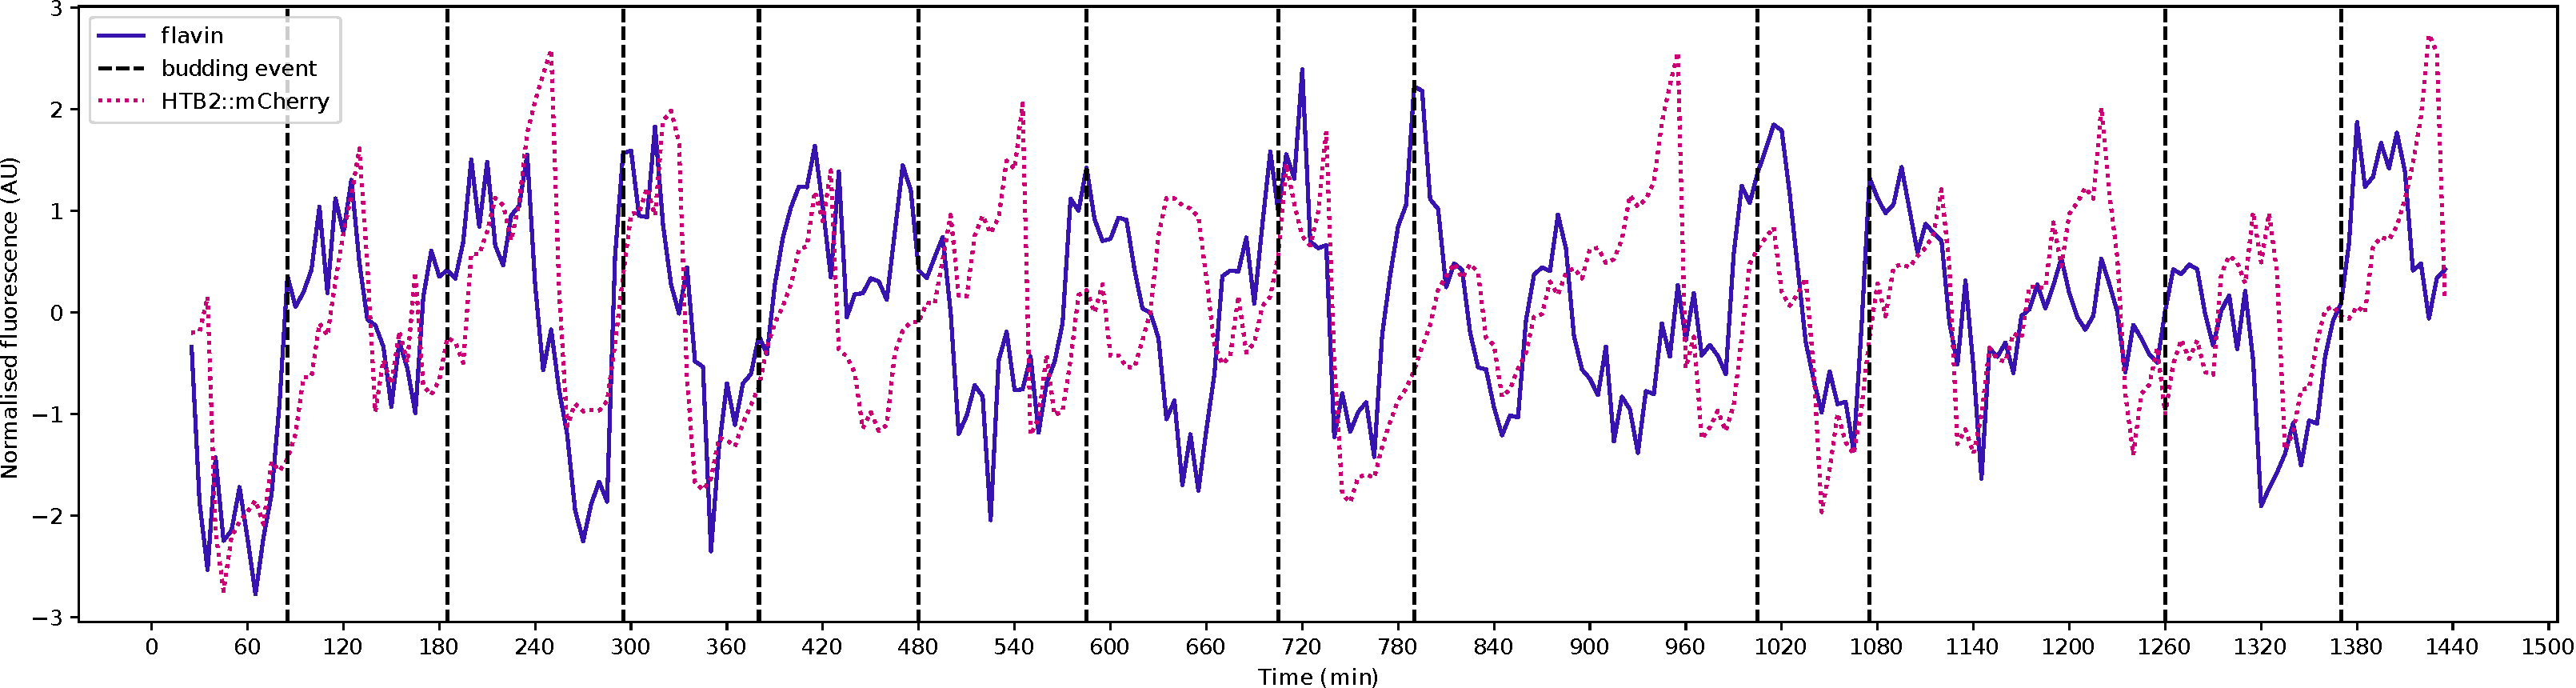
\includegraphics[width=1.0\linewidth]{single_birth_plot_edit.pdf}
    \caption{
      Flavin fluorescence (blue, solid lines) and histone 2B (orange, dotted lines) levels in a single, representative FY4 HTB2::mCherry cell grown in \SI{20}{\gram~\litre^{-1}} glucose.
      Vertical lines (black, dashed) indicate budding events.
      Star ($\star$) shows a flavin oscillation without a corresponding cell division cycle.
    }
  \label{fig:biology-highglc-single}
\end{figure}


\begin{figure}
  \centering
    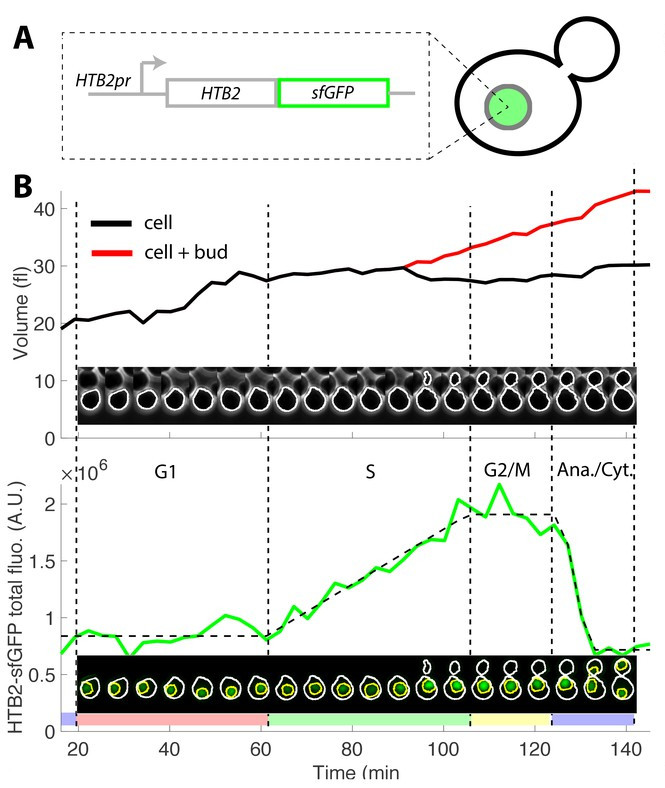
\includegraphics[width=0.5\linewidth]{garmendia-torresMultipleInputsEnsure2018_1_adapted.jpg}
    \caption{
      \textbf{(A)} Engineering a fluorescent protein cassette fused to \textit{HTB2} \textbf{(B)} allows the identification of phases of the cell division cycle by modelling the fluorescent protein intensity changes over time as piecewise linear sections.
      Adapted from \textcite{garmendia-torresMultipleInputsEnsure2018}.
    }
  \label{fig:biology-htb2}
\end{figure}

To show that metabolic cycles are generated autonomously and are coupled to the cell division cycle, I replicated the single-cell flavin oscillations observed by \textcite{baumgartnerFlavinbasedMetabolicCycles2018} that supported these observations.
Replicating results from a previous flavin-based microfluidics study is important to confirm that the microfluidics set-up I used truly monitored the yeast metabolic cycle, especially if the set-up differed from previous studies \parencite{papagiannakisAutonomousMetabolicOscillations2017, baumgartnerFlavinbasedMetabolicCycles2018}.

Fig.\ \ref{fig:biology-highglc-single} shows that oscillations in flavin fluorescence peak when a bud forms in GS/M, as evidenced by prototrophic FY4 HTB2::mCherry cells grown in minimal medium supplemented with \SI{20}{\gram~\litre^{-1}} glucose.
The HTB2::mCherry insertion allows monitoring phases of the cell division cycle via imaging and quantifying the intensity of the inserted fluorescent protein (Fig.\ \ref{fig:biology-htb2}), while also allowing monitoring flavin fluorescence by avoiding overlap of emission spectra.

As observed, oxidation of flavin upon budding was expected for these reasons:
\begin{enumerate}
  \item Flavin fluorescence peaks (oxidised form) and NAD(P)H fluorescence peaks (reduced form) at the same time in chemostat cultures \parencite{murrayRedoxRegulationRespiring2011}.
  \item NAD(P)H is in the reduced form when buds form \parencite{papagiannakisAutonomousMetabolicOscillations2017}.
  \item The flavoprotein lipoamide dehydrogenase is in redox equilibrium with NAD(P)H \parencite{sianoNADHFlavinFluorescence1989}.
\end{enumerate}

Fig.\ \ref{fig:biology-highglc-single} also shows that in some cases, a metabolic oscillation occurred without cell division cycle progression or bud formation.
Such cases, also revealed by \textcite{papagiannakisAutonomousMetabolicOscillations2017} via NAD(P)H cycles, confirmed that the metabolic cycle is generated autonomously from the cell division cycle.


\begin{figure}
  \centering
  \begin{subfigure}[htpb]{0.45\textwidth}
   \centering
   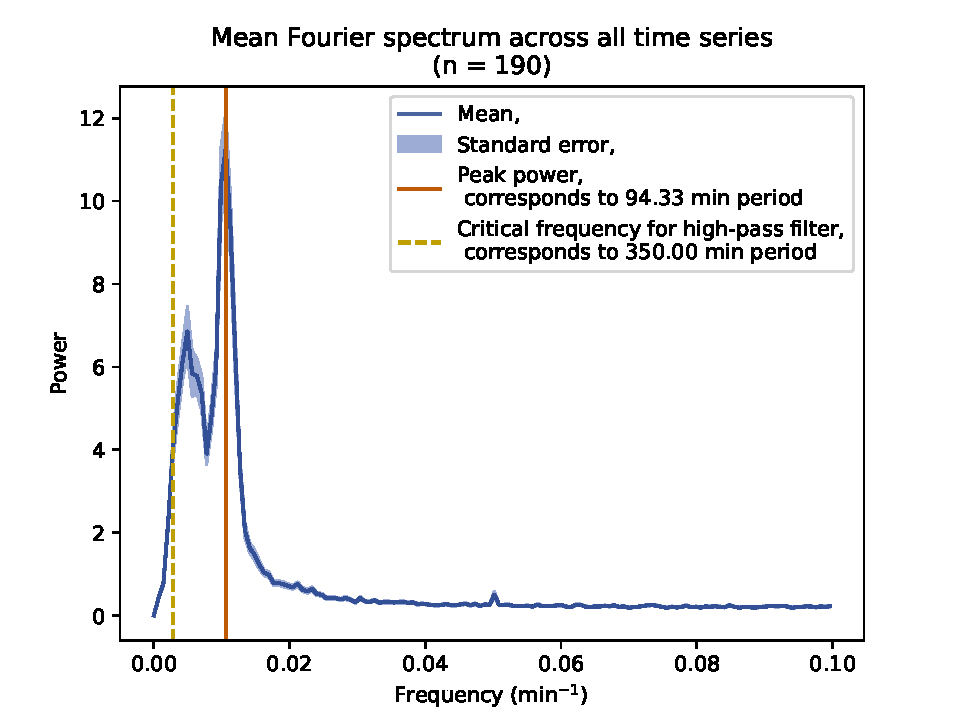
\includegraphics[width=\textwidth]{htb2mCherry_26643_14}
   \caption{
   }
   \label{fig:biology-highglc-sync-fourier}
  \end{subfigure}%
  \begin{subfigure}[htpb]{0.45\textwidth}
   \centering
   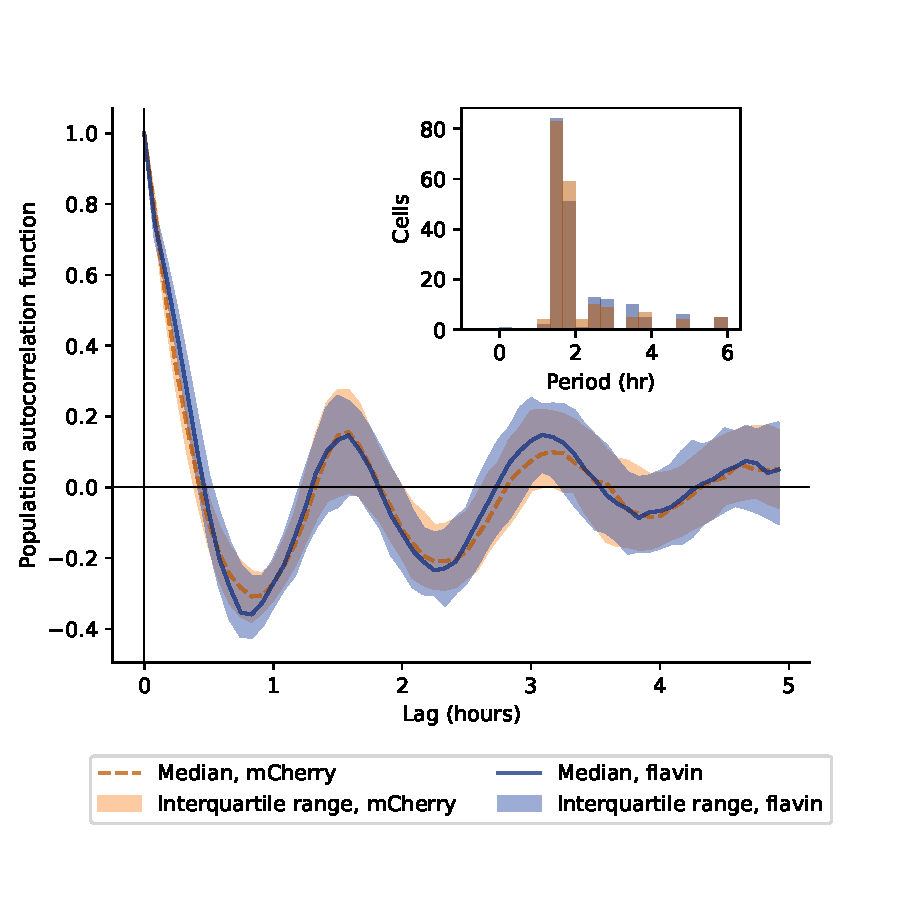
\includegraphics[width=\textwidth]{htb2mCherry_26643_12}
   \caption{
   }
   \label{fig:biology-highglc-sync-acf}
  \end{subfigure}

  \caption{
    \textbf{(\ref{fig:biology-highglc-sync-fourier})} Mean Fourier spectrum of flavin fluorescence across cells; \textbf{(\ref{fig:biology-highglc-sync-acf})} median autocorrelation functions of flavin fluorescence (blue) and histone 2B levels (orange) time series, along with \textit{\textbf{(inset)}} the periods of each oscillator across cells as determined by the frequency with the greatest power in each signal's Fourier spectrum.
    Data are from FY4 HTB2::mCherry cells under \SI{20}{\gram~\litre^{-1}} glucose.
  }
  \label{fig:biology-highglc-sync-spectral}
\end{figure}

To quantify the period of the oscillators, I used several time series analysis methods in concert.
Fig.\ \ref{fig:biology-highglc-sync-spectral} shows that the mean Fourier spectrum and median autocorrelation function both suggest that flavin fluorescence oscillated at a period of $\approx$\SI{90}{\minute}.
Fig.\ \ref{fig:biology-highglc-sync-acf} additionally shows that the cell division cycle proceeds at the same frequency, as evidenced by the autocorrelation function of mCherry.
This periodicity agrees with the literature regarding the duration of the cell division cycle in such permissive growth conditions. % [CITATIONS NEEDED]


\begin{figure}
  \centering
  \begin{subfigure}[htpb]{0.45\textwidth}
   \centering
   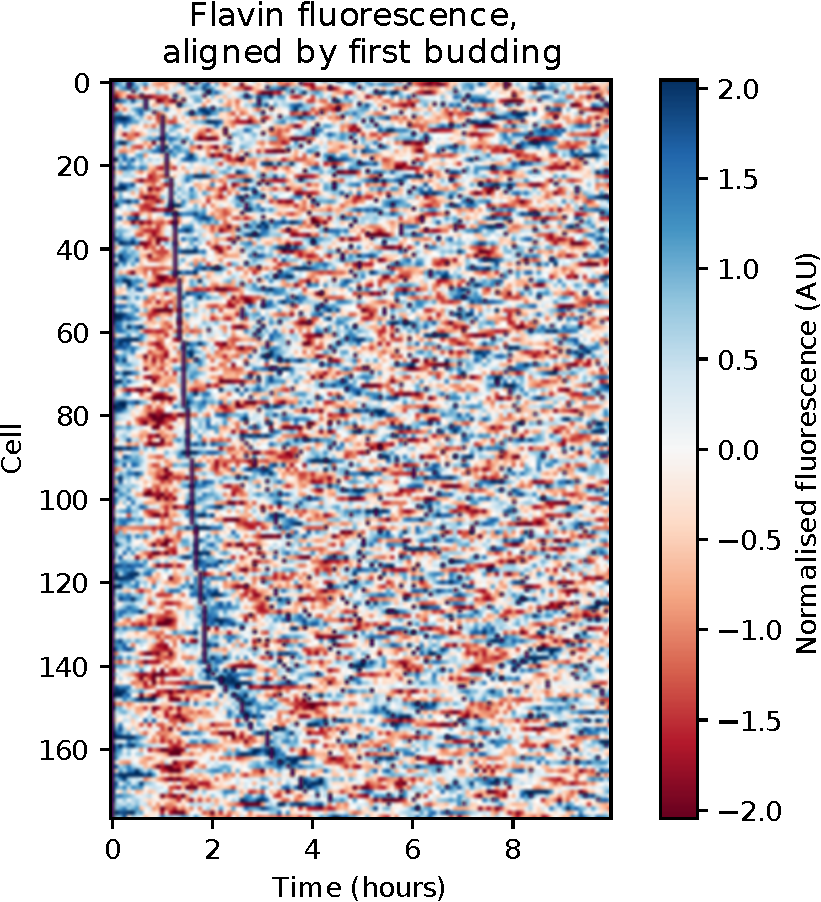
\includegraphics[width=\textwidth]{heatmap_edit.pdf}
   \caption{
   }
   \label{fig:biology-highglc-sync-heatmap}
  \end{subfigure}%
  \begin{subfigure}[htpb]{0.45\textwidth}
   \centering
   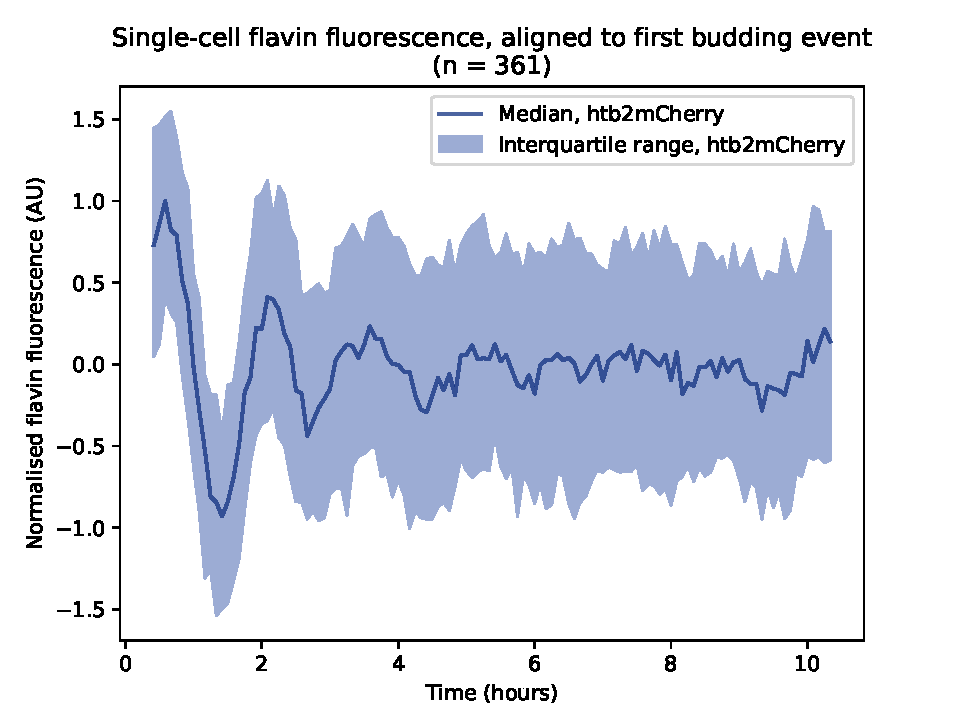
\includegraphics[width=\textwidth]{htb2mCherry_26643_6}
   \caption{
   }
   \label{fig:biology-highglc-sync-median}
  \end{subfigure}

  \begin{subfigure}[htpb]{0.45\textwidth}
   \centering
   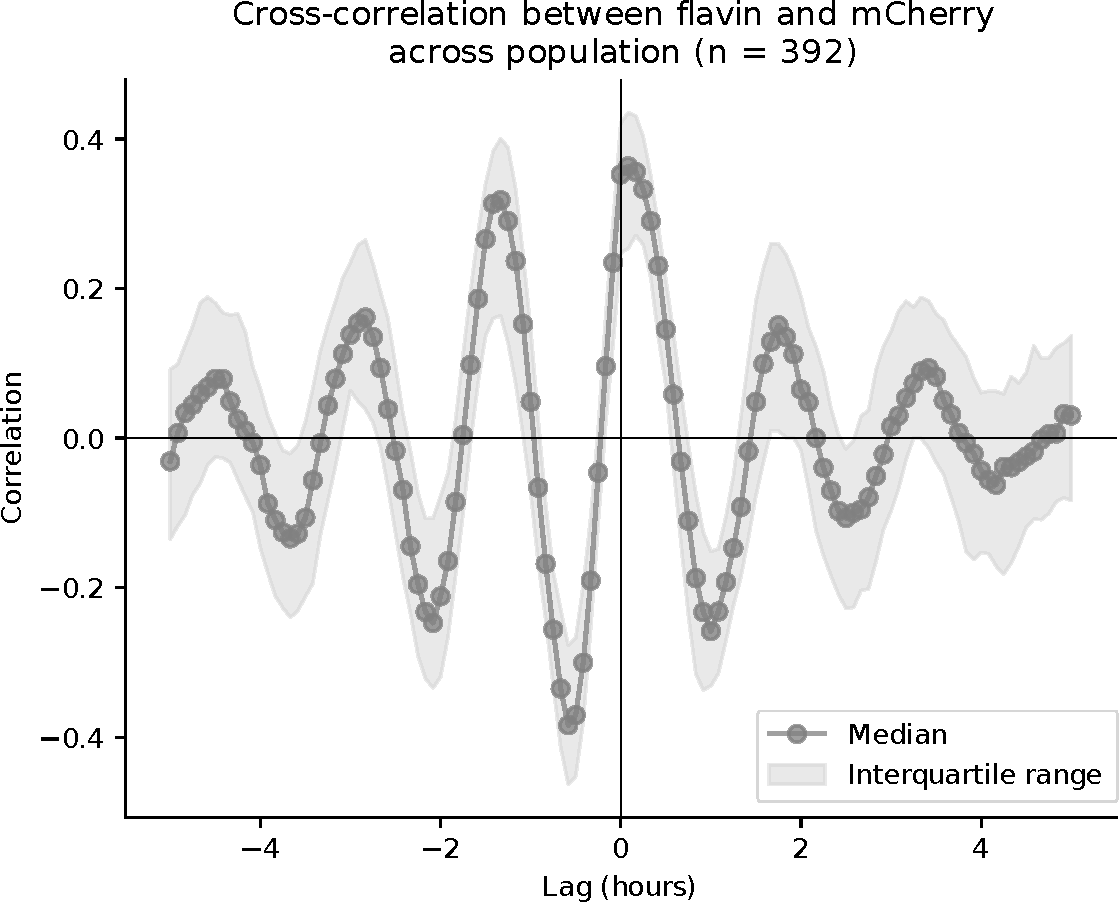
\includegraphics[width=\textwidth]{xcf_edit.pdf}
   \caption{
   }
   \label{fig:biology-highglc-sync-xcf}
  \end{subfigure}

  \caption{
    \textbf{(\ref{fig:biology-highglc-sync-heatmap})}
    Heatmap showing the flavin fluorescence (pixels on a red-blue scale) and budding events (black pixels) of each cell,
    signals are aligned by the first budding event;
    \textbf{(\ref{fig:biology-highglc-sync-median})}
    median flavin fluorescence signal across cells, aligned to first budding event; and
    \textbf{(\ref{fig:biology-highglc-sync-xcf})}
    median cross-correlation function between flavin and histone 2B signals.
    Data are from FY4 HTB2::mCherry cells in \SI{20}{\gram~\litre^{-1}} glucose.
  }
  \label{fig:biology-highglc-sync-corr}
\end{figure}

To visualise the relationship between the metabolic cycle and the cell division cycle,
Fig.\ \ref{fig:biology-highglc-sync-corr} shows that
budding events synchronise with peaks in fluorescence and
that the cell division cycle varies between cells,
but most are just under \SI{2}{\hour}, agreeing with Fig.\ \ref{fig:biology-highglc-sync-acf} (inset).
The oscillatory shape of the median (Fig.\ \ref{fig:biology-highglc-sync-median}) further confirms the synchrony between the metabolic cycle and budding events.

Finally, to quantify the relationship between the metabolic cycle and the cell division cycle, I computed the cross-correlation function between the flavin and mCherry signals across the population (Fig.\ \ref{fig:biology-highglc-sync-xcf}).
This function shows that the mCherry signals are, on average, shifted by \SI{5}{\minute} relative to the flavin signals.


%\section[Abrupt nutrient changes]{Cells autonomously generate flavin oscillations, independently of the cell division cycle, in response to abrupt nutrient changes.}
\section{Decoupling between the metabolic and cell division cycles}
\label{sec:biology-abrupt}

\begin{figure}
  \centering
  \begin{subfigure}[htpb]{1.0\textwidth}
   \centering
   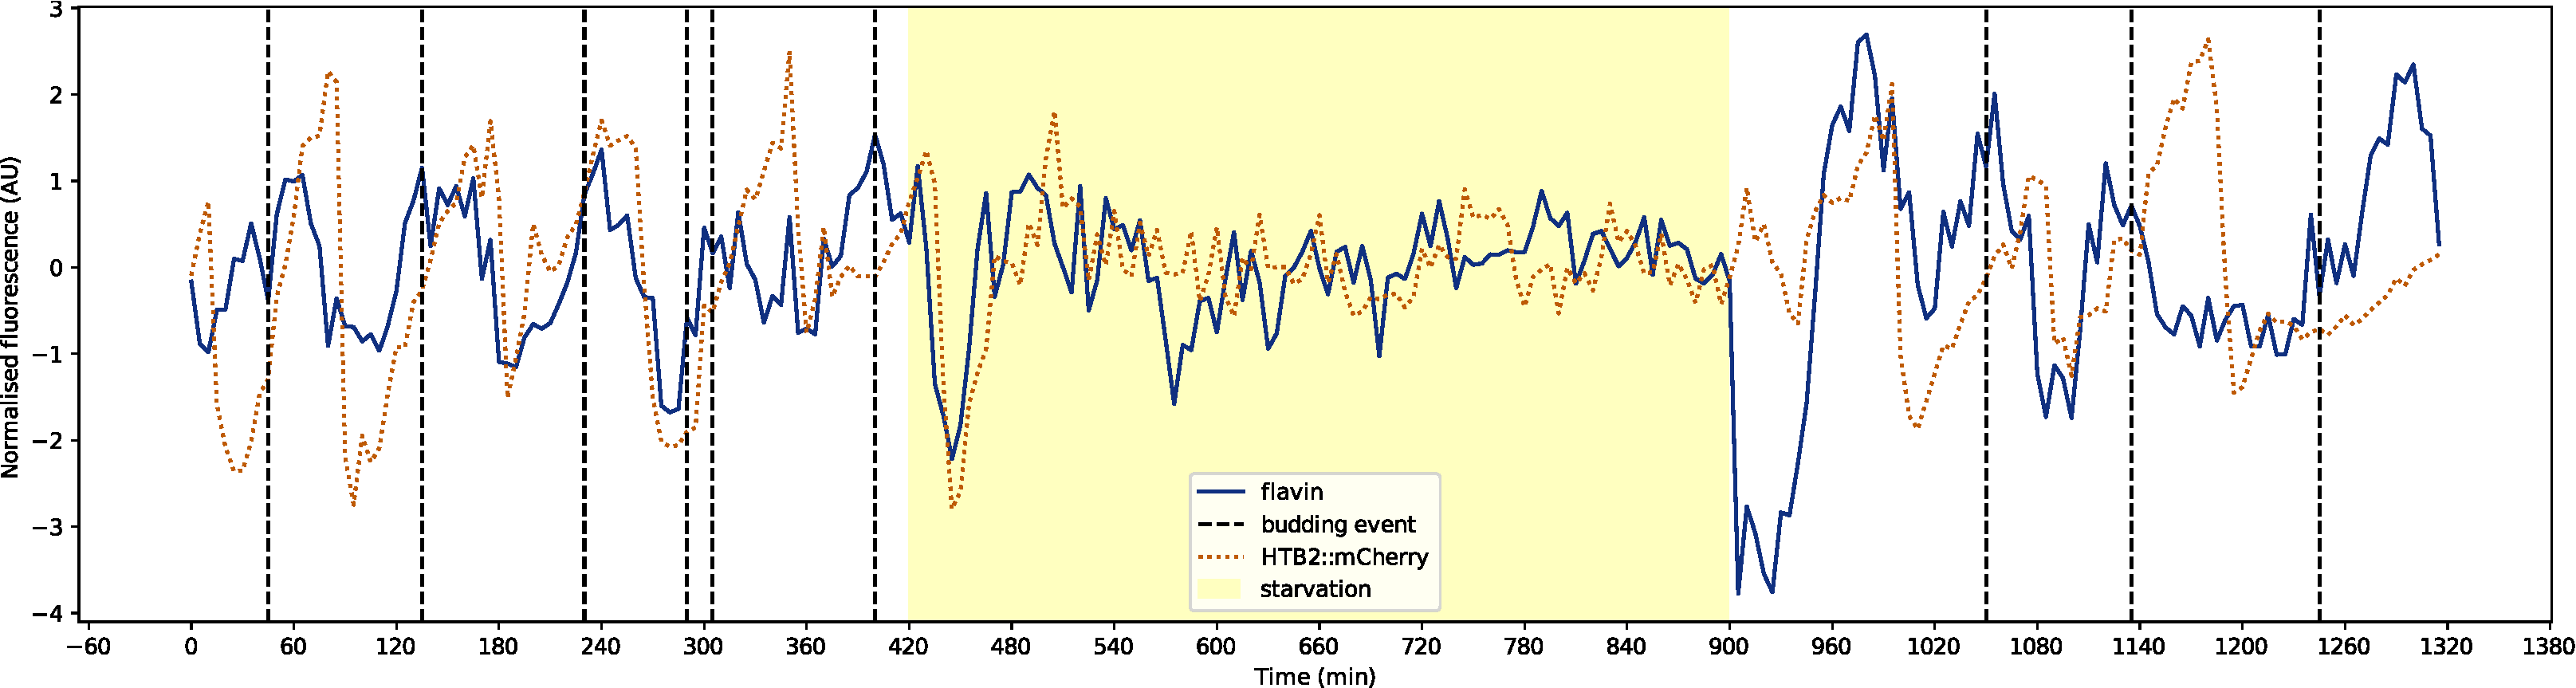
\includegraphics[width=\textwidth]{starvation_single_birth_plot_new_edit.pdf}
   \caption{
   }
   \label{fig:biology-starvation-single}
  \end{subfigure}

  \begin{subfigure}[htpb]{0.9\textwidth}
   \centering
   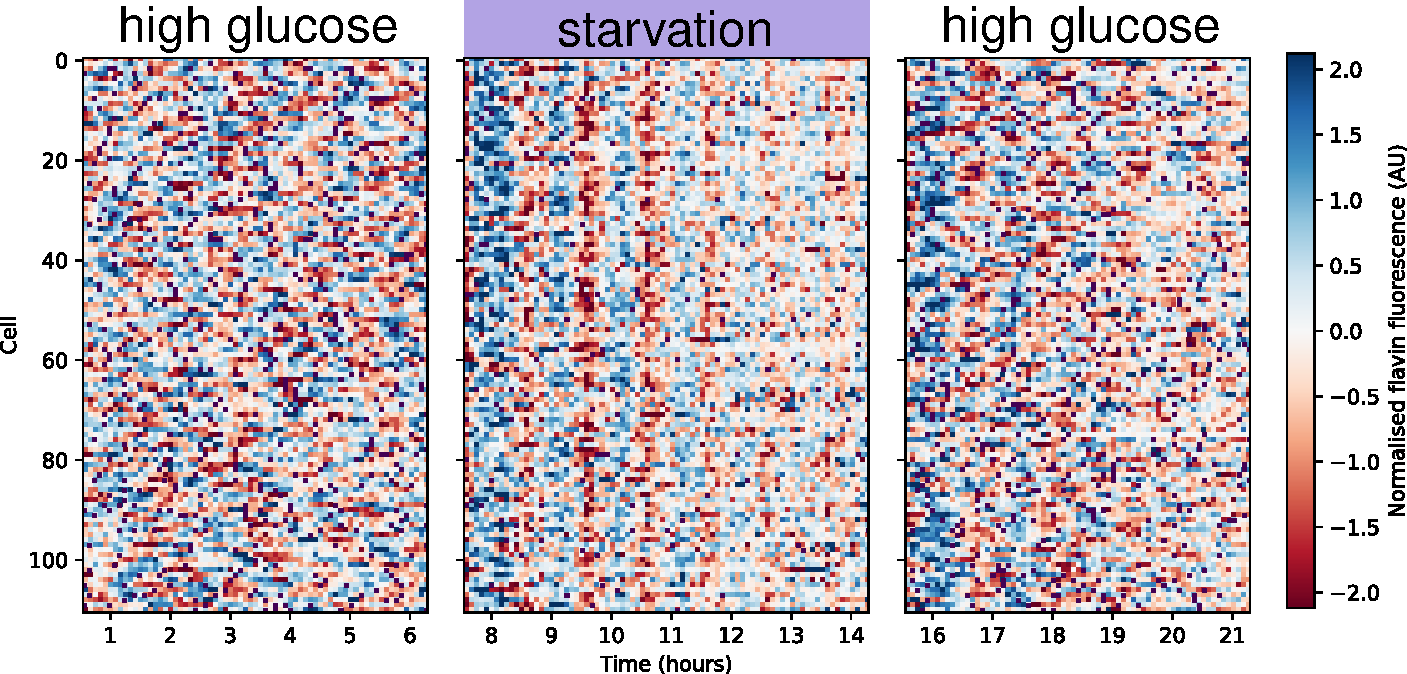
\includegraphics[width=\textwidth]{heatmap_012_edit.pdf}
   \caption{
   }
   \label{fig:biology-starvation-heatmap}
  \end{subfigure}

  \caption{
    \textbf{(\ref{fig:biology-starvation-single})}
    Flavin fluorescence (blue, solid lines) and histone 2B (orange, dotted lines) levels in a single, representative FY4 HTB2::mCherry cell.
    Vertical lines (black, dashed) indicate budding events.
    Shading indicates the glucose starvation period.
    \textbf{(\ref{fig:biology-starvation-heatmap})}
    Heatmap showing the flavin fluorescence (pixels on a red-blue scale) and budding events (black pixels) of each cell.
    Data are from FY4 and HTB2::mCherry cells, subject to \SI{7.5}{\gram~\litre^{-1}} glucose for \SI{7}{\hour} before being abruptly switched to \SI{0}{\gram~\litre^{-1}} glucose for \SI{8}{\hour} and then resumed to \SI{7.5}{\gram~\litre^{-1}} glucose for \SI{7}{\hour}.
  }
  \label{fig:biology-starvation}
\end{figure}

To provide additional evidence that cells generate metabolic oscillations independent of the cell division cycle, I created a condition in which cells do not undergo cell division.
Specifically, I did so by inducing starvation: I cultured FY4 and HTB2::mCherry cells in \SI{7.5}{\gram~\litre^{-1}} glucose for \SI{7}{\hour} before being abruptly switched to \SI{0}{\gram~\litre^{-1}} glucose for \SI{8}{\hour} and then resumed to \SI{7.5}{\gram~\litre^{-1}} glucose for \SI{7}{\hour} (Fig.\ \ref{fig:biology-starvation}).
This abrupt induction of starvation is similar to experiments described by \textcite{bagameryPutativeBetHedgingStrategy2020} that showed the heterogeneity of cellular responses to starvation.


\begin{figure}
  \centering
  \begin{subfigure}[htpb]{0.45\textwidth}
   \centering
   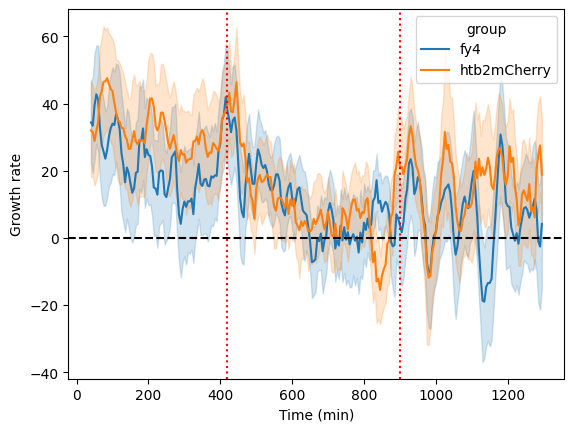
\includegraphics[width=\textwidth]{allstrains_19972_gr}
   \caption{
   }
   \label{fig:biology-starvation-gr}
  \end{subfigure}%
  \begin{subfigure}[htpb]{0.45\textwidth}
   \centering
   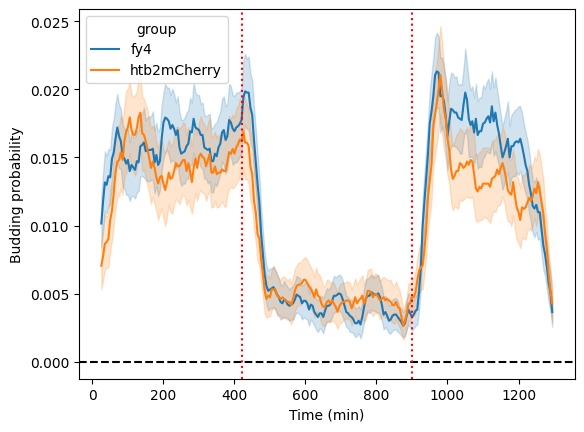
\includegraphics[width=\textwidth]{allstrains_19972_budprob}
   \caption{
   }
   \label{fig:biology-starvation-budprob}
  \end{subfigure}

  \caption{
    \textbf{(\ref{fig:biology-starvation-gr})}
    Mean growth rate and
    \textbf{(\ref{fig:biology-starvation-budprob})}
    budding probability of FY4 (blue) and HTB2::mCherry (orange) strains over time during the glucose-starvation experiment, with 95\% confidence intervals shown (shaded).
    Vertical lines (red) show changes in nutrient media.
  }
  \label{fig:biology-starvation-gr-budprob}
\end{figure}

Fig.\ \ref{fig:biology-starvation} shows that when cells are in high glucose, oscillations were asynchronous, consistent with section~\ref{sec:biology-sync}, \textcite{papagiannakisAutonomousMetabolicOscillations2017} and \textcite{baumgartnerFlavinbasedMetabolicCycles2018}.
When cells grown in high glucose were abruptly starved of glucose, their flavin oscillations reset phase.
During starvation, these flavin oscillations continue, while growth rate drops and budding events are sparse (Fig.\ \ref{fig:biology-starvation-gr-budprob}).

% Does this paragraph belong in the discussion?
The results show that metabolic oscillations may be generated when cell division cycle is halted, providing strong evidence that the metabolic cycle is generated autonomously and independently of the cell division cycle.
In addition, the results show that each cell can individually reset the phase of its metabolic cycle in response to abrupt changes in environmental conditions; similar phenomena have been observed upon bulk addition of carbon sources \parencite{kuangMsn2RegulateExpression2017, krishnaMinimalPushPull2018}.
Importantly, the results suggest that diffusion of signalling chemicals between cells is not required for generation of metabolic cycles.
Combined with results from the previous section, my results suggest that the metabolic cycle responds to external conditions and create windows of opportunity for initiating the cell division cycle that the cell can choose not to take if conditions are not favourable.


\begin{figure}
  \centering
  \begin{subfigure}[htpb]{1.0\textwidth}
   \centering
   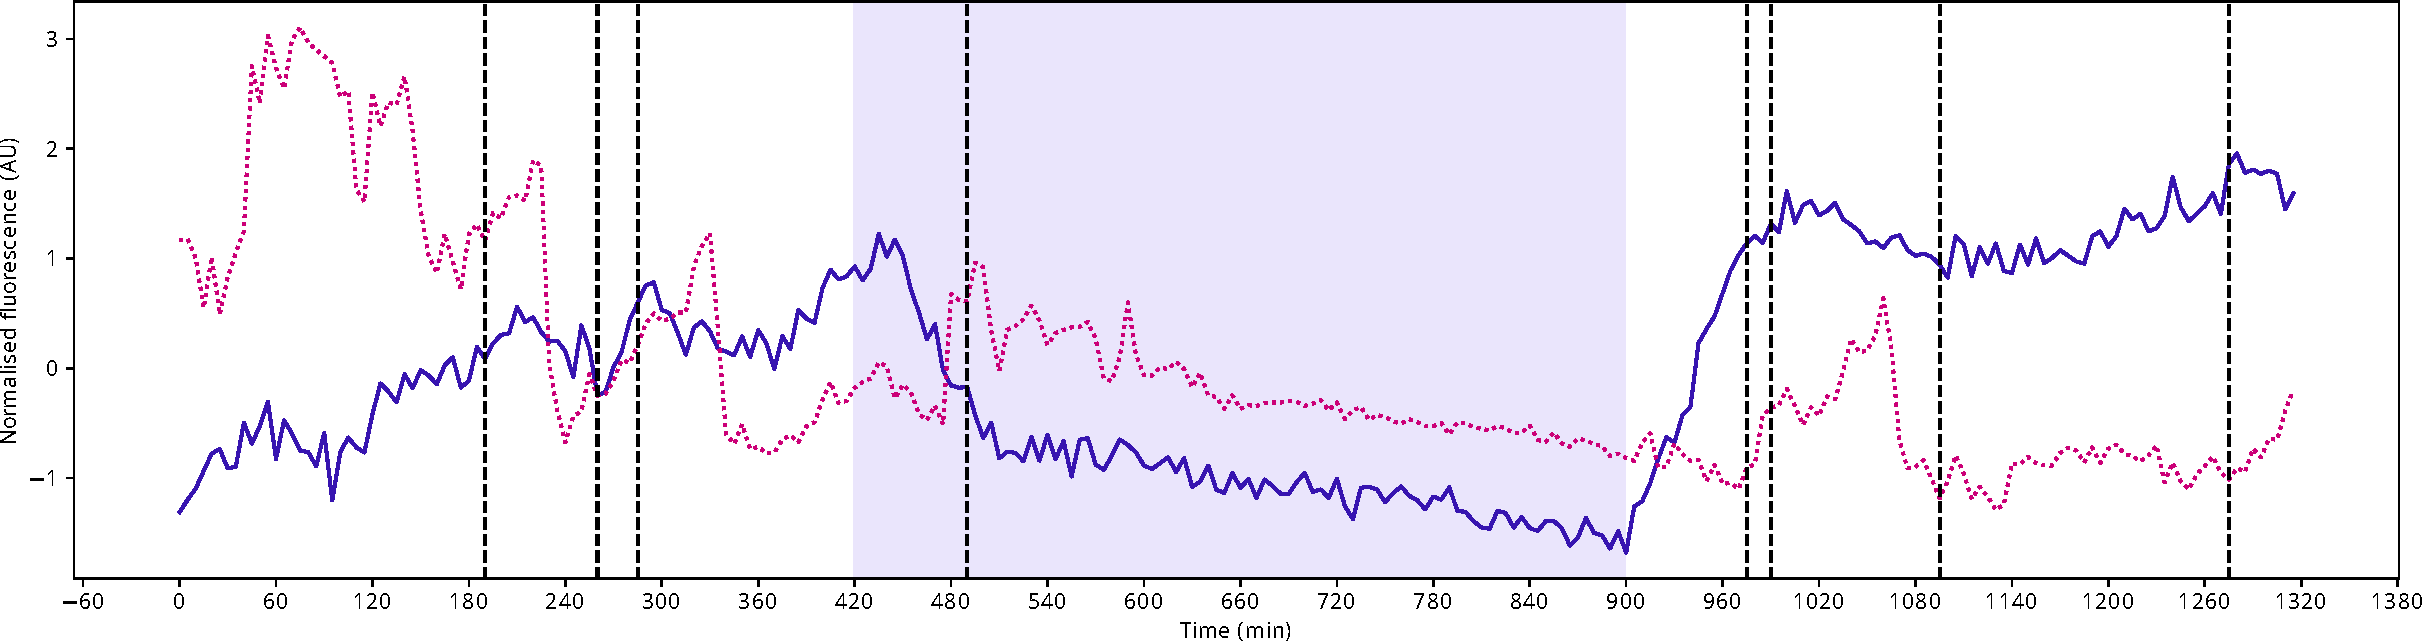
\includegraphics[width=\textwidth]{starvation_raw_13-39-01.pdf}
   \caption{
   }
   \label{fig:biology-starvation-raw-2}
  \end{subfigure}

  \begin{subfigure}[htpb]{1.0\textwidth}
   \centering
   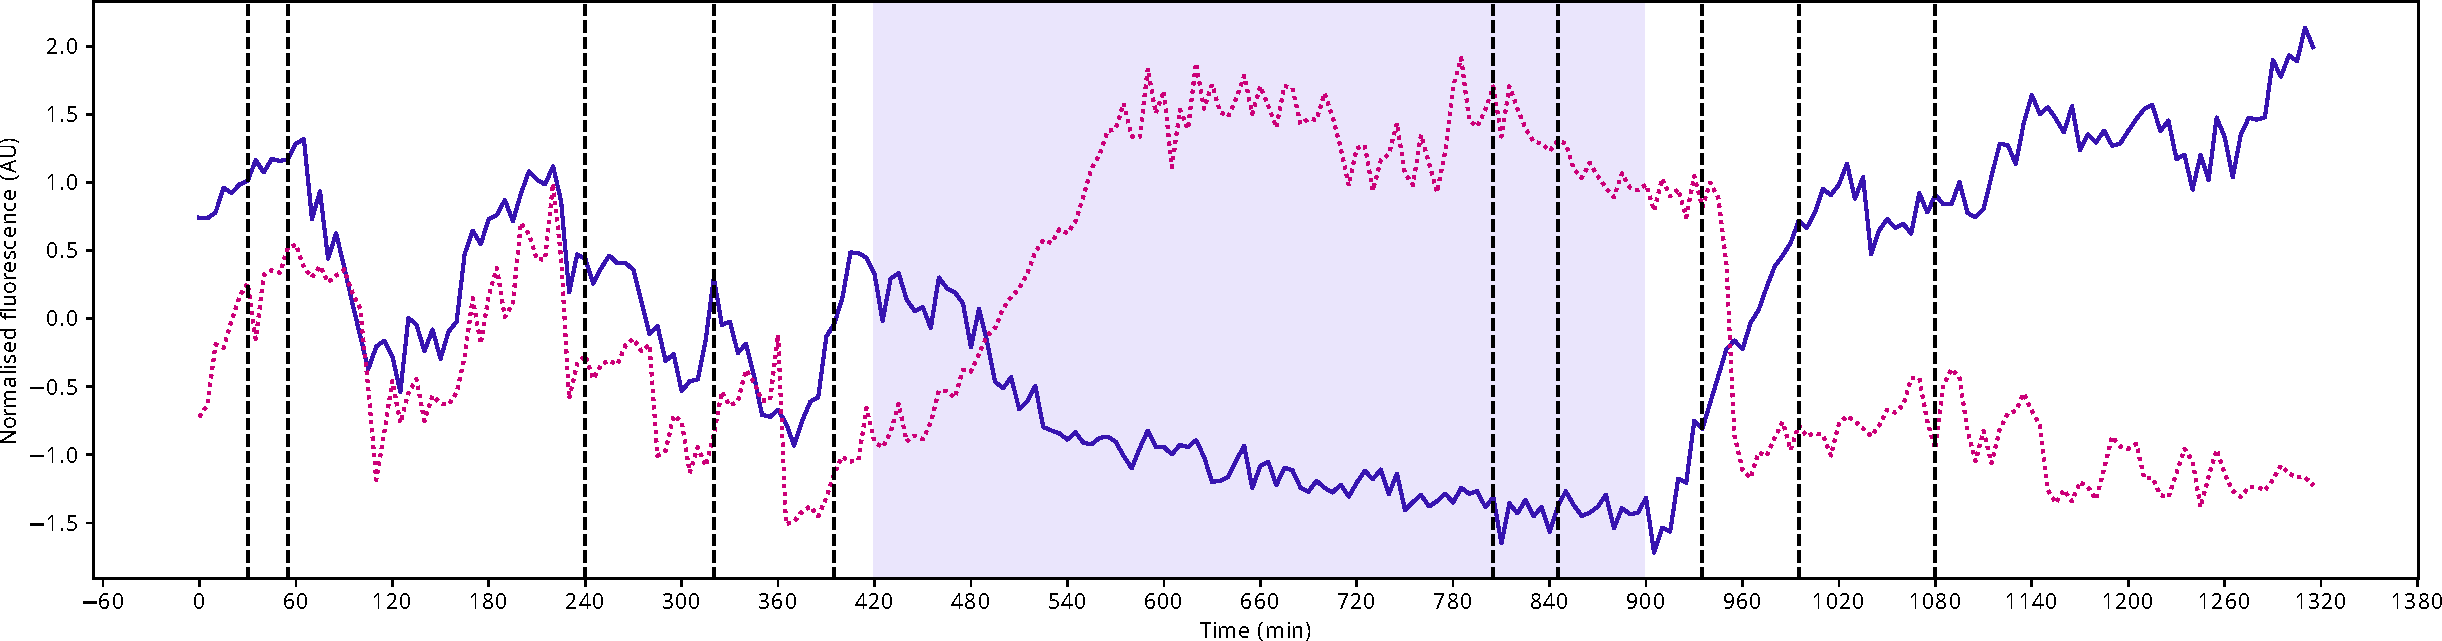
\includegraphics[width=\textwidth]{starvation_raw_13-07-02.pdf}
   \caption{
   }
   \label{fig:biology-starvation-raw-1}
  \end{subfigure}

  \caption{
    Flavin fluorescence (blue, solid lines) and histone 2B (orange, dotted lines) levels in two FY4 HTB2::mCherry cells in the glucose starvation experiment; vertical lines (black, dashed) indicate budding events.
    \textbf{(\ref{fig:biology-starvation-raw-2})} is an example of a cell with a low intensity of mCherry during starvation, while \textbf{(\ref{fig:biology-starvation-raw-1})} is an example with a high intensity of mCherry.
    Unlike other figures, the flavin and mCherry time series were normalised to give a mean of 0 and standard deviation of 1 so that they can be plot on the same vertical axes, but the high-pass Butterworth filter was not applied to emphasise the trajectories of raw values.
  }
  \label{fig:biology-starvation-raw}
\end{figure}


\begin{figure}
  \centering
  
\includegraphics[width=0.7\textwidth]{placeholder01.pdf}
  \caption{
    Insert caption here.
    This is the heatmap/histogram for the glucose starvation experiment.
  }
  \label{fig:biology-starvation-histogram}
\end{figure}

The model in which the metabolic cycle creates windows of opportunity for the cell division cycle implies that, upon starvation, cell division cycles progress to the next gap phase (G1 or G2) while the metabolic cycle continues.
To test this implication, Fig.\ \ref{fig:biology-starvation-raw} shows that cells may remain in G1 (Fig.\ \ref{fig:biology-starvation-raw-2}), as evidenced by low mCherry intensity, or G2 (Fig.\ \ref{fig:biology-starvation-raw-1}), as evidenced by high mCherry intensity.
Extending this investigation across a population of cells, Fig.\ \ref{fig:biology-starvation-heatmap} shows that (INSERT INTERPRETATION OF NEW HEATMAP HERE...).

(INSERT 1--2 PARAGRAPHS OF INTERPRETATION OF NEW HEATMAP)


\section{Metabolic cycles in different genetic backgrounds}
\label{sec:biology-backgrounds}

\begin{figure}
  \centering
  \begin{subfigure}[htpb]{0.45\textwidth}
   \centering
   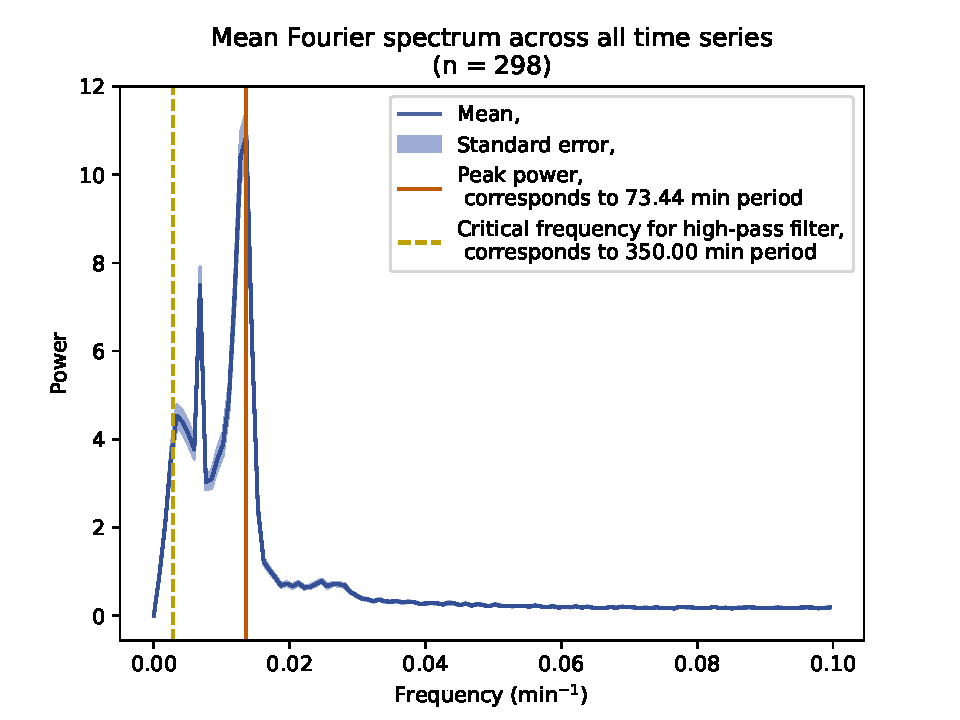
\includegraphics[width=\textwidth]{by4741_491_13}
   \caption{
   }
   \label{fig:biology-by4741-sync-fourier}
  \end{subfigure}%
  \begin{subfigure}[htpb]{0.45\textwidth}
   \centering
   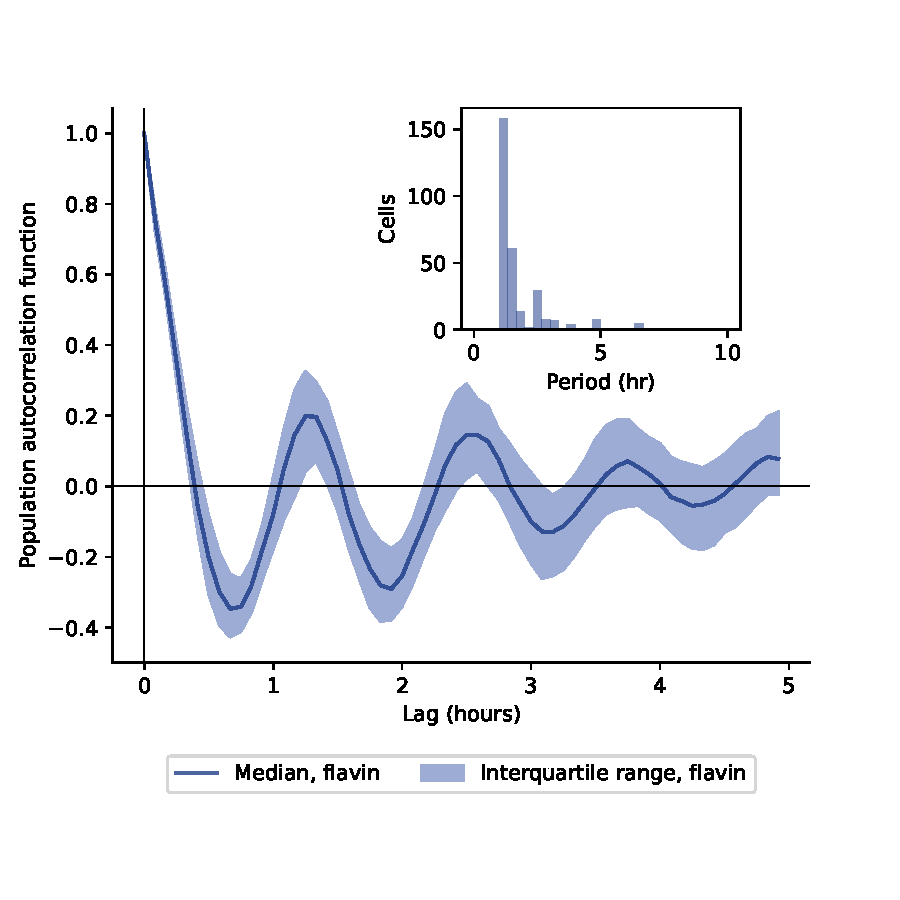
\includegraphics[width=\textwidth]{by4741_491_12}
   \caption{
   }
   \label{fig:biology-by4741-sync-acf}
  \end{subfigure}

  \begin{subfigure}[htpb]{0.45\textwidth}
   \centering
   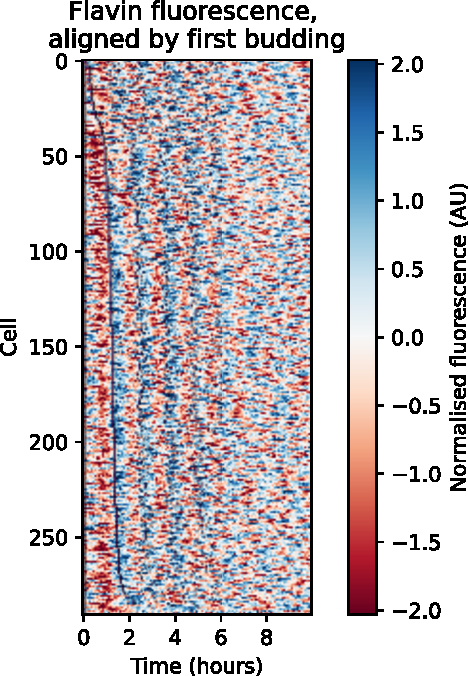
\includegraphics[width=\textwidth]{by4741_491_7.pdf}
   \caption{
   }
   \label{fig:biology-by4741-sync-heatmap}
  \end{subfigure}%
  \begin{subfigure}[htpb]{0.45\textwidth}
   \centering
   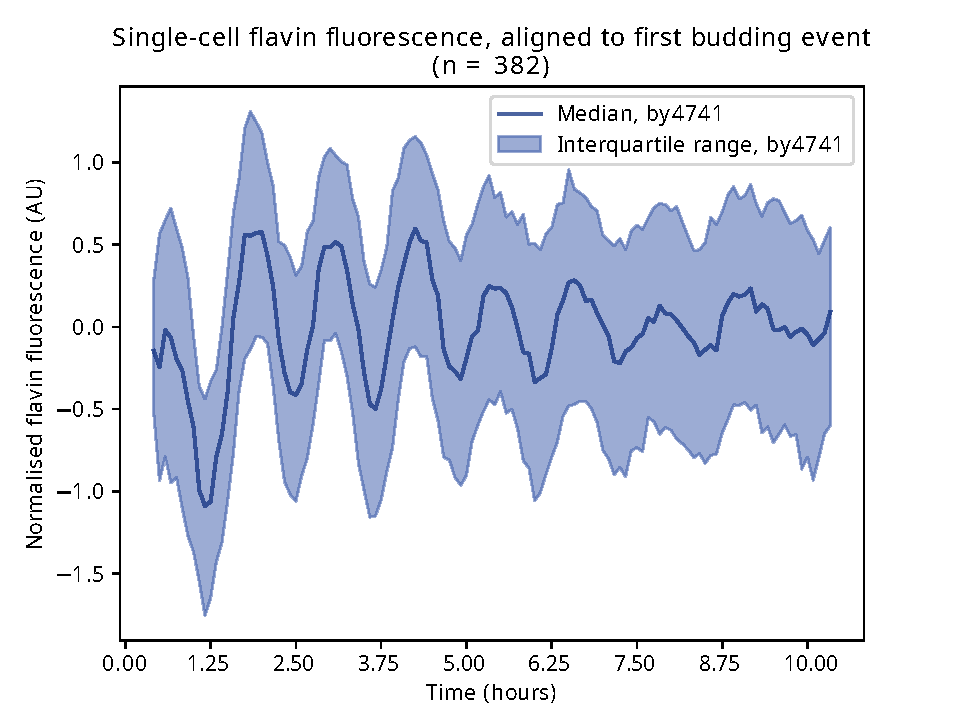
\includegraphics[width=\textwidth]{by4741_491_6}
   \caption{
   }
   \label{fig:biology-by4741-sync-median}
  \end{subfigure}

  \caption{
    \textbf{(\ref{fig:biology-by4741-sync-fourier})} Mean Fourier spectrum of flavin fluorescence across cells; \textbf{(\ref{fig:biology-by4741-sync-acf})} median autocorrelation function of flavin fluorescence time series, along with \textit{\textbf{(inset)}} the periods of each oscillator across cells as determined by the frequency with the greatest power in each signal's Fourier spectrum;
    \textbf{(\ref{fig:biology-by4741-sync-heatmap})}
    heatmap showing the flavin fluorescence (pixels on a red-blue scale) and budding events (black pixels) of each cell,
    signals are aligned by the first budding event; and
    \textbf{(\ref{fig:biology-by4741-sync-median})}
    median flavin fluorescence signal across cells, aligned to first budding event.
    Data are from BY4741 cells in \SI{10}{\gram~\litre^{-1}} glucose.
  }
  \label{fig:biology-by4741-sync}
\end{figure}

To show that the metabolic cycle is robust,
I monitored flavin autofluorescence signals from the auxotrophic BY4741 strain, grown in minimal medium supplemented with uracil and the amino acids required for this strain to grow, plus \SI{10}{\gram~\litre^{-1}} glucose.
Showing that metabolic cycles occur in an auxotroph is important because it shows that many cellular aspects must be impaired for the cycle to disappear, supporting the idea that the metabolic cycle is an intrinsic property of budding yeast.
Similar to FY4 HTB2::mCherry cells, BY4741 cells show robust, consistent oscillations in flavin fluorescence that peak upon budding (figure~\ref{fig:biology-by4741-sync}), although metabolic cycles have a period of $\approx$\SI{75}{\minute} in this case.
The shorter period, implying a higher growth rate, may be explained by a lack of burden caused by a lack of an mCherry insertion, and by media supplements.
% Discussion (probably in discussion section at the end): to be 'proper', I should perform an experiment with the BY4741 HTB2::mCherry I engineered.


\begin{figure}
  \centering
  \begin{subfigure}[htpb]{0.45\textwidth}
   \centering
   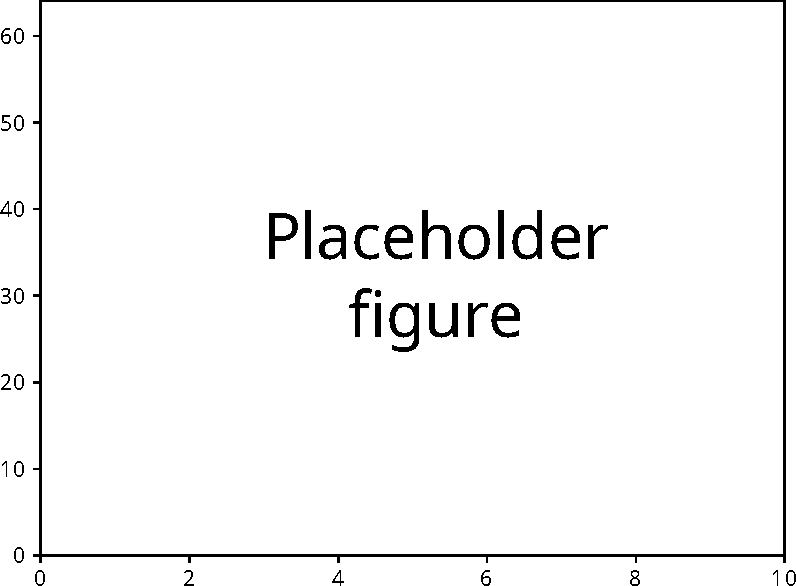
\includegraphics[width=\textwidth]{placeholder03.pdf}
   \caption{
   }
   \label{fig:biology-cenpk-sync-fourier}
  \end{subfigure}%
  \begin{subfigure}[htpb]{0.45\textwidth}
   \centering
   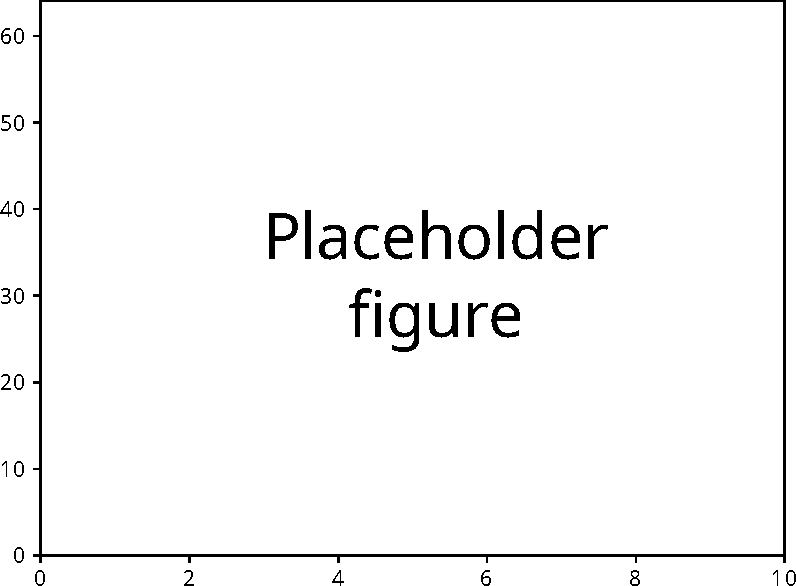
\includegraphics[width=\textwidth]{placeholder03.pdf}
   \caption{
   }
   \label{fig:biology-cenpk-sync-acf}
  \end{subfigure}

  \begin{subfigure}[htpb]{0.45\textwidth}
   \centering
   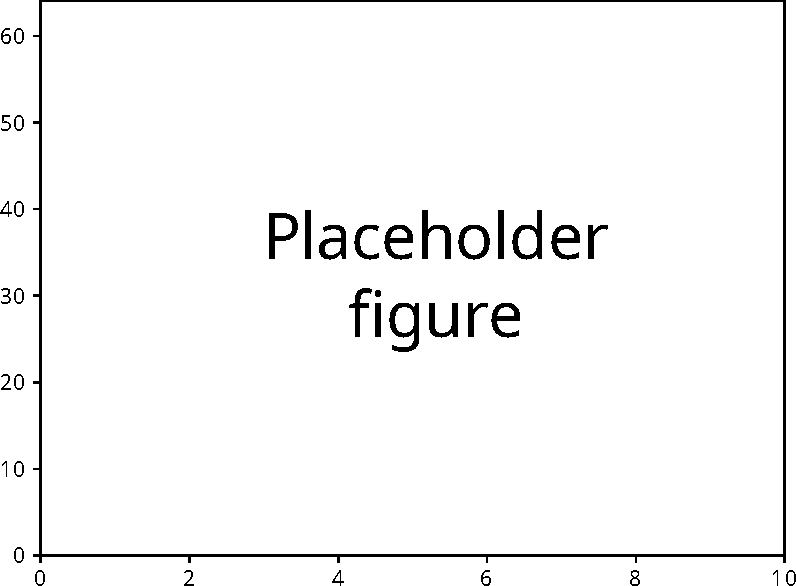
\includegraphics[width=\textwidth]{placeholder03.pdf}
   \caption{
   }
   \label{fig:biology-cenpk-sync-heatmap}
  \end{subfigure}%
  \begin{subfigure}[htpb]{0.45\textwidth}
   \centering
   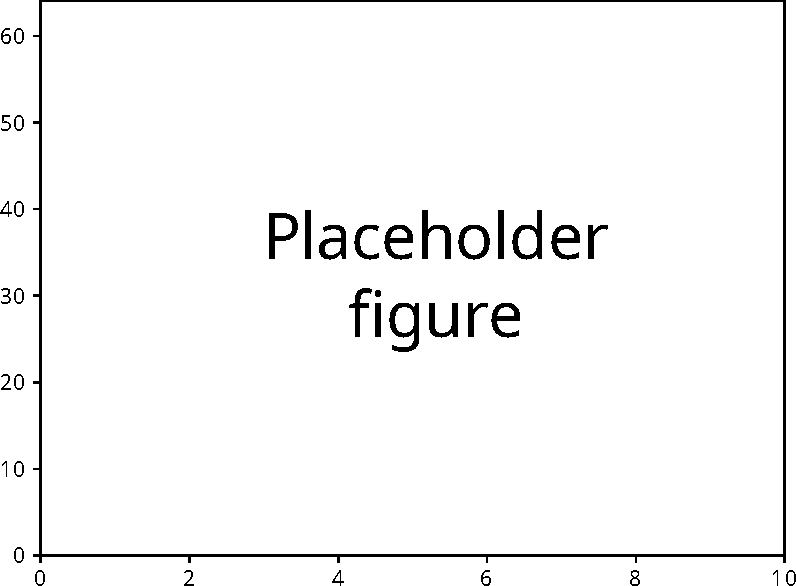
\includegraphics[width=\textwidth]{placeholder03.pdf}
   \caption{
   }
   \label{fig:biology-cenpk-sync-median}
  \end{subfigure}

  \caption{
    \textbf{(\ref{fig:biology-cenpk-sync-fourier})} Mean Fourier spectrum of flavin fluorescence across cells; \textbf{(\ref{fig:biology-cenpk-sync-acf})} median autocorrelation function of flavin fluorescence time series, along with \textit{\textbf{(inset)}} the periods of each oscillator across cells as determined by the frequency with the greatest power in each signal's Fourier spectrum;
    \textbf{(\ref{fig:biology-cenpk-sync-heatmap})}
    heatmap showing the flavin fluorescence (pixels on a red-blue scale) and budding events (black pixels) of each cell,
    signals are aligned by the first budding event; and
    \textbf{(\ref{fig:biology-cenpk-sync-median})}
    median flavin fluorescence signal across cells, aligned to first budding event.
    Data are from CEN.PK cells in \SI{10}{\gram~\litre^{-1}} glucose.
  }
  \label{fig:biology-cenpk-sync}
\end{figure}

(INSERT CEN.PK FIGURE AND DISCUSSION HERE.)


\section{Metabolic cycles in different carbon sources}
\label{sec:biology-carbon}

To extend on the idea that the metabolic cycle responds to nutrient conditions and accordingly adjusts the cell's metabolism and cell division cycle, I performed experiments in which I culture cells in pyruvate and in a growth-limiting glucose concentration.
These experiments are important as they confirm conclusions about varying nutrient conditions made by \textcite{papagiannakisAutonomousMetabolicOscillations2017},
% TODO: Fact-check
but using flavin autofluorescence and in additional carbon sources.
Specifically, pyruvate provided an example of a non-fermentable carbon source to test whether the switch from fermentative to respiratory metabolism affected the metabolic cycle.
Additionally, a growth-limiting glucose concentration emulated low-glucose concentrations in a chemostat and was thus used to test whether long YMCs observed in such conditions can be replicated in a microfluidics platform.

\begin{figure}
  \centering
  \begin{subfigure}[htpb]{1.0\textwidth}
   \centering
   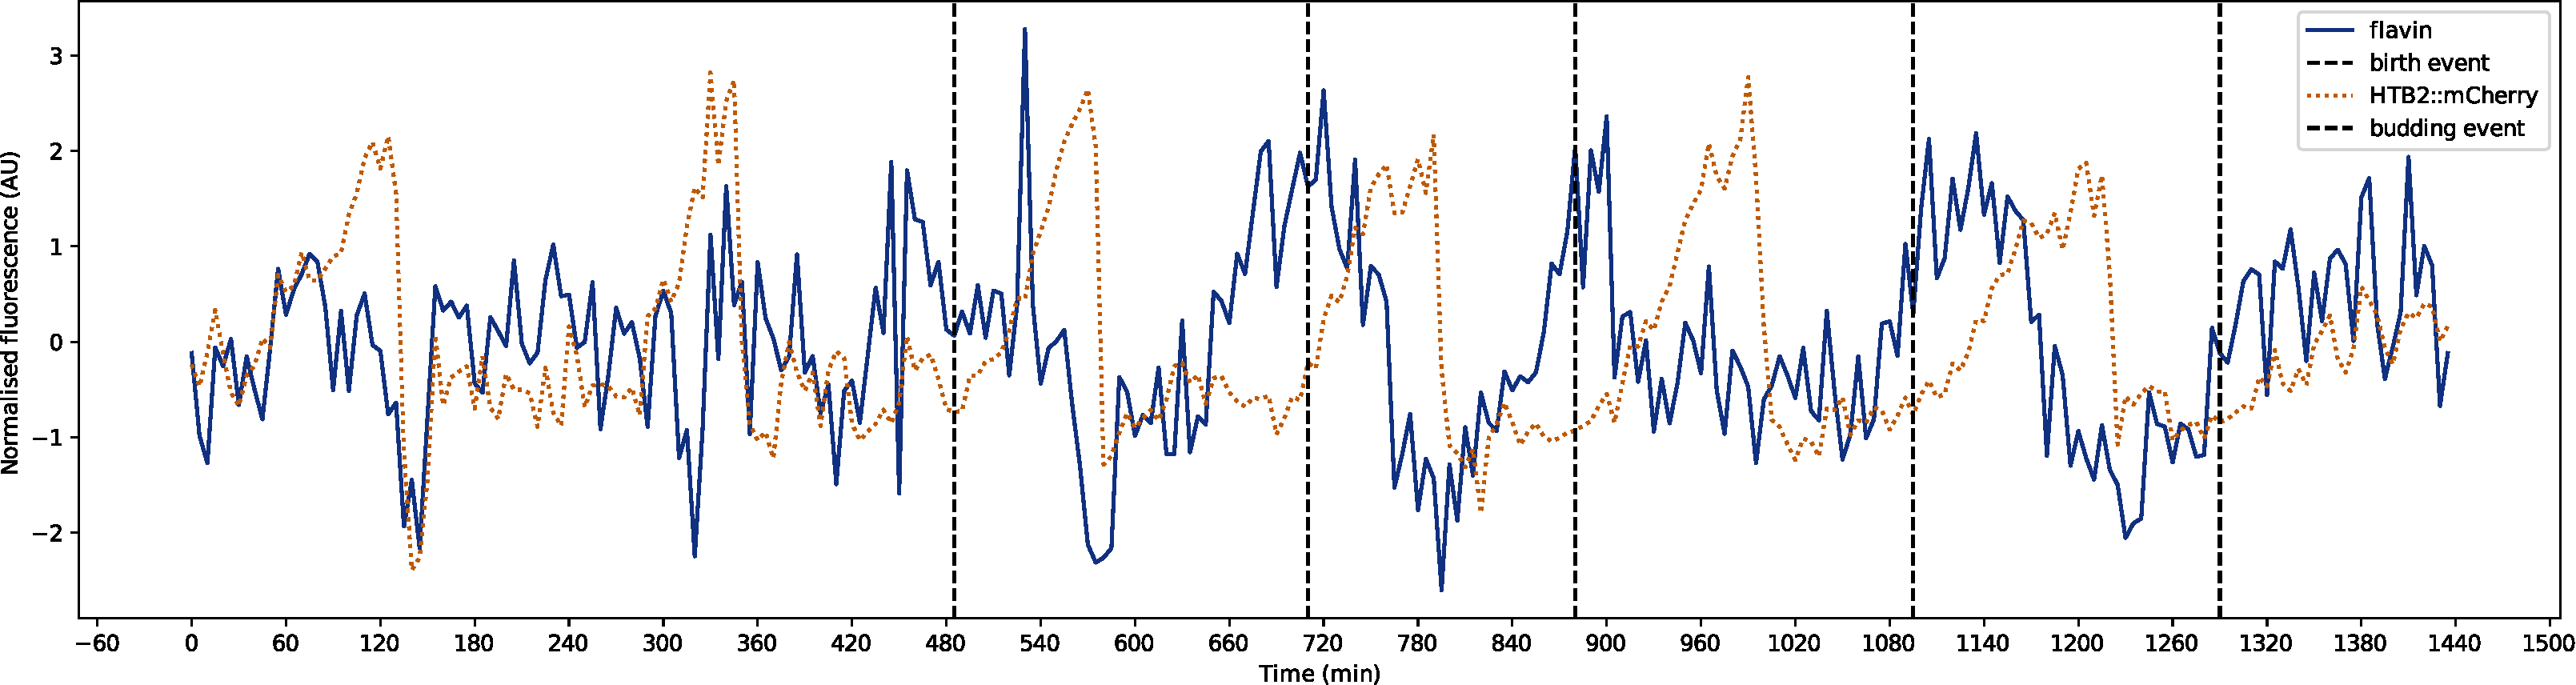
\includegraphics[width=\textwidth]{pyruvate_single_birth_plot_edit.pdf}
   \caption{
     % Oscillations of flavin fluorescence lengthen when cells are cultivated in \SI{20}{\gram~\litre^{-1}} pyruvate while the duration of S/M phase stays constant.
     %Figure shows sample flavin fluorescence levels (purple) and histone 2B localisation (pink) in single cells.
     %Vertical lines (black) indicate budding.
   }
   \label{fig:biology-pyruvate-single}

  \end{subfigure}
  \begin{subfigure}[t]{0.45\textwidth}
   \centering
   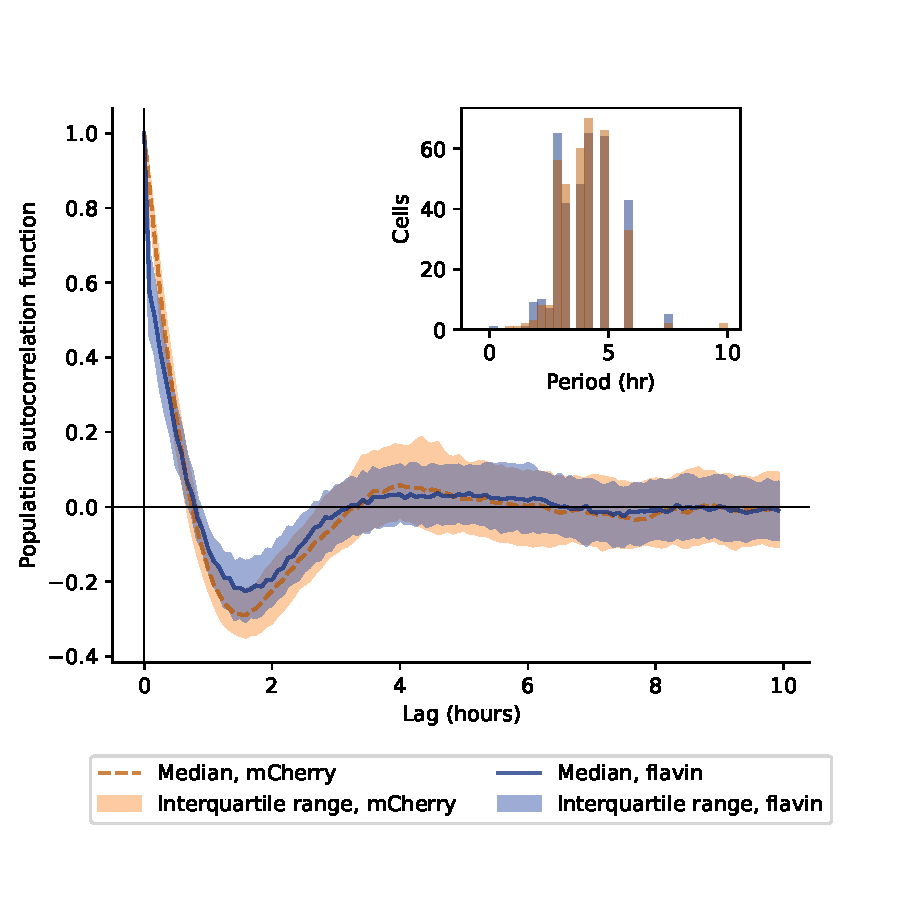
\includegraphics[width=\textwidth]{htb2mCherry_31594_12.pdf}
   \caption{
     % Autocorrelation functions and periods determined by Fourier spectrum of flavin fluorescence and histone 2B levels.
     % This figure indicates that the cells' metabolic cycles and cell division cycles are both consistently approximately 4 hours long.
   }
   \label{fig:biology-pyruvate-acf}
  \end{subfigure}%
  \begin{subfigure}[t]{0.45\textwidth}
   \centering
   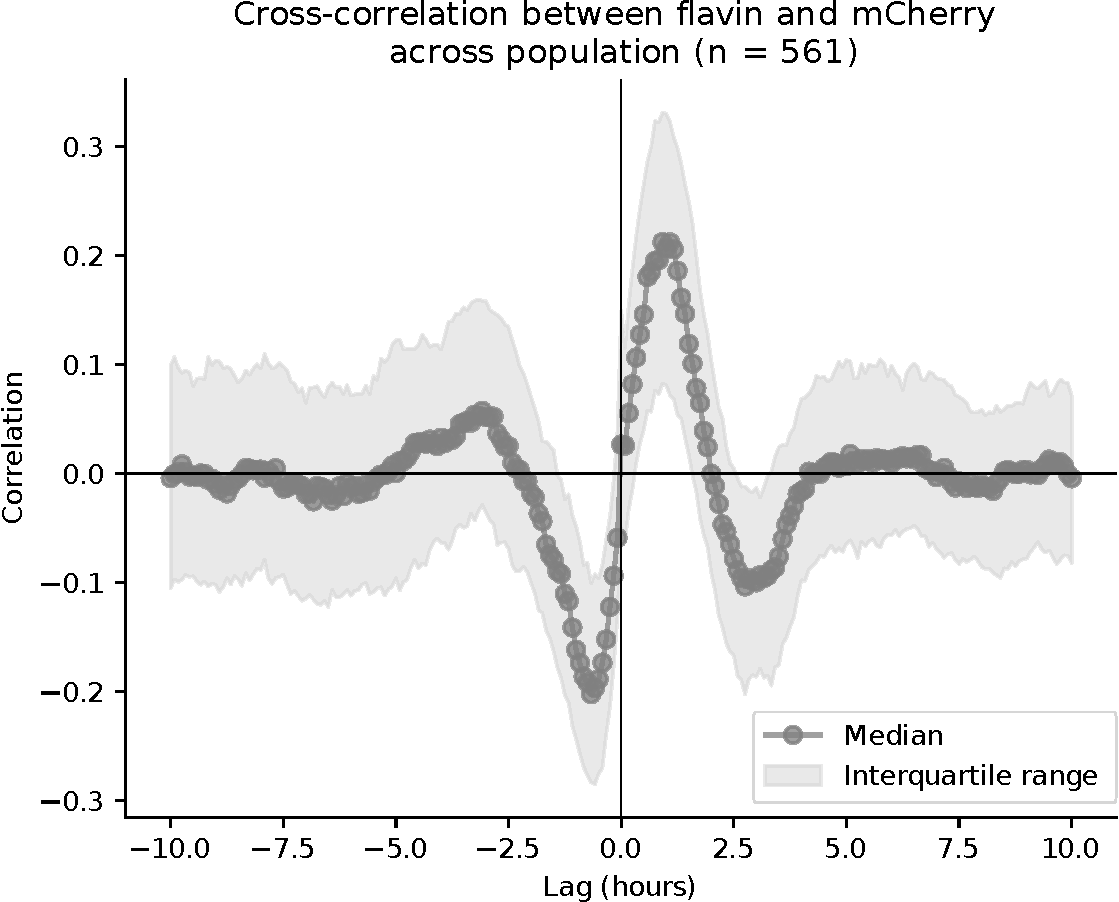
\includegraphics[width=\textwidth]{pyruvate_xcf_edit.pdf}
   \caption{
    %Cross-correlation between flavin and histone 2B signals, indicating that histone levels peak 1 hour after flavin fluorescence peaks.
   }
   \label{fig:biology-pyruvate-xcf}
  \end{subfigure}

  \caption{
    \textbf{(\ref{fig:biology-pyruvate-single})}
    Flavin fluorescence (blue, solid lines) and histone 2B (orange, dotted lines) levels in a single, representative FY4 HTB2::mCherry cell grown in \SI{20}{\gram~\litre^{-1}} pyruvate.
    Vertical lines (black, dashed) indicate budding events.
    \textbf{(\ref{fig:biology-pyruvate-acf})}
    Median autocorrelation functions of flavin fluorescence (blue) and histone 2B levels (orange) time series, along with \textit{\textbf{(inset)}} the periods of each oscillator across cells as determined by the frequency with the greatest power in each signal's Fourier spectrum.
    \textbf{(\ref{fig:biology-pyruvate-xcf})}
    Median cross-correlation function between flavin and histone 2B signals.
    Data are from FY4 HTB2::mCherry cells in \SI{20}{\gram~\litre^{-1}} pyruvate.
  }
  \label{fig:biology-pyruvate}
\end{figure}

Fig.\ \ref{fig:biology-pyruvate} shows that FY4 HTB2::mCherry cells showed longer metabolic cycles and cell division cycles, of approximately \SI{4}{\hour}, when grown in minimal media supplemented with \SI{20}{\gram~\litre^{-1}} pyruvate.
In addition, there were more cases in which the flavin signal peaks without a budding event. %(supplementary figure ...).
Furthermore, the synchrony between the two oscillators remained, but with a longer lag of the cell division cycle with respect to the metabolic cycle (Fig.\ \ref{fig:biology-pyruvate-xcf}).
Figure~\ref{fig:biology-pyruvate-single} shows that the longer cell division cycles were because of longer G1 phases but unchanged S/M phases, as evidenced by the longer flat regions of the HTB2::mCherry signal.
However, the flavin cycles were not regular over long periods of time, as evidenced by a lack of repeated oscillations in the cross-correlation function.

% COULD DO:
% (Add statistical tests to reject the null hypothesis that the mean duration of metabolic cycles in pyruvate is equal to the mean duration of metabolic cycles in high glucose.  This would depend on having a good number of the duration, and it looks like the inset is the best candidate for this.)


\begin{figure}
  \centering
  \begin{subfigure}[htpb]{1.0\textwidth}
   \centering
   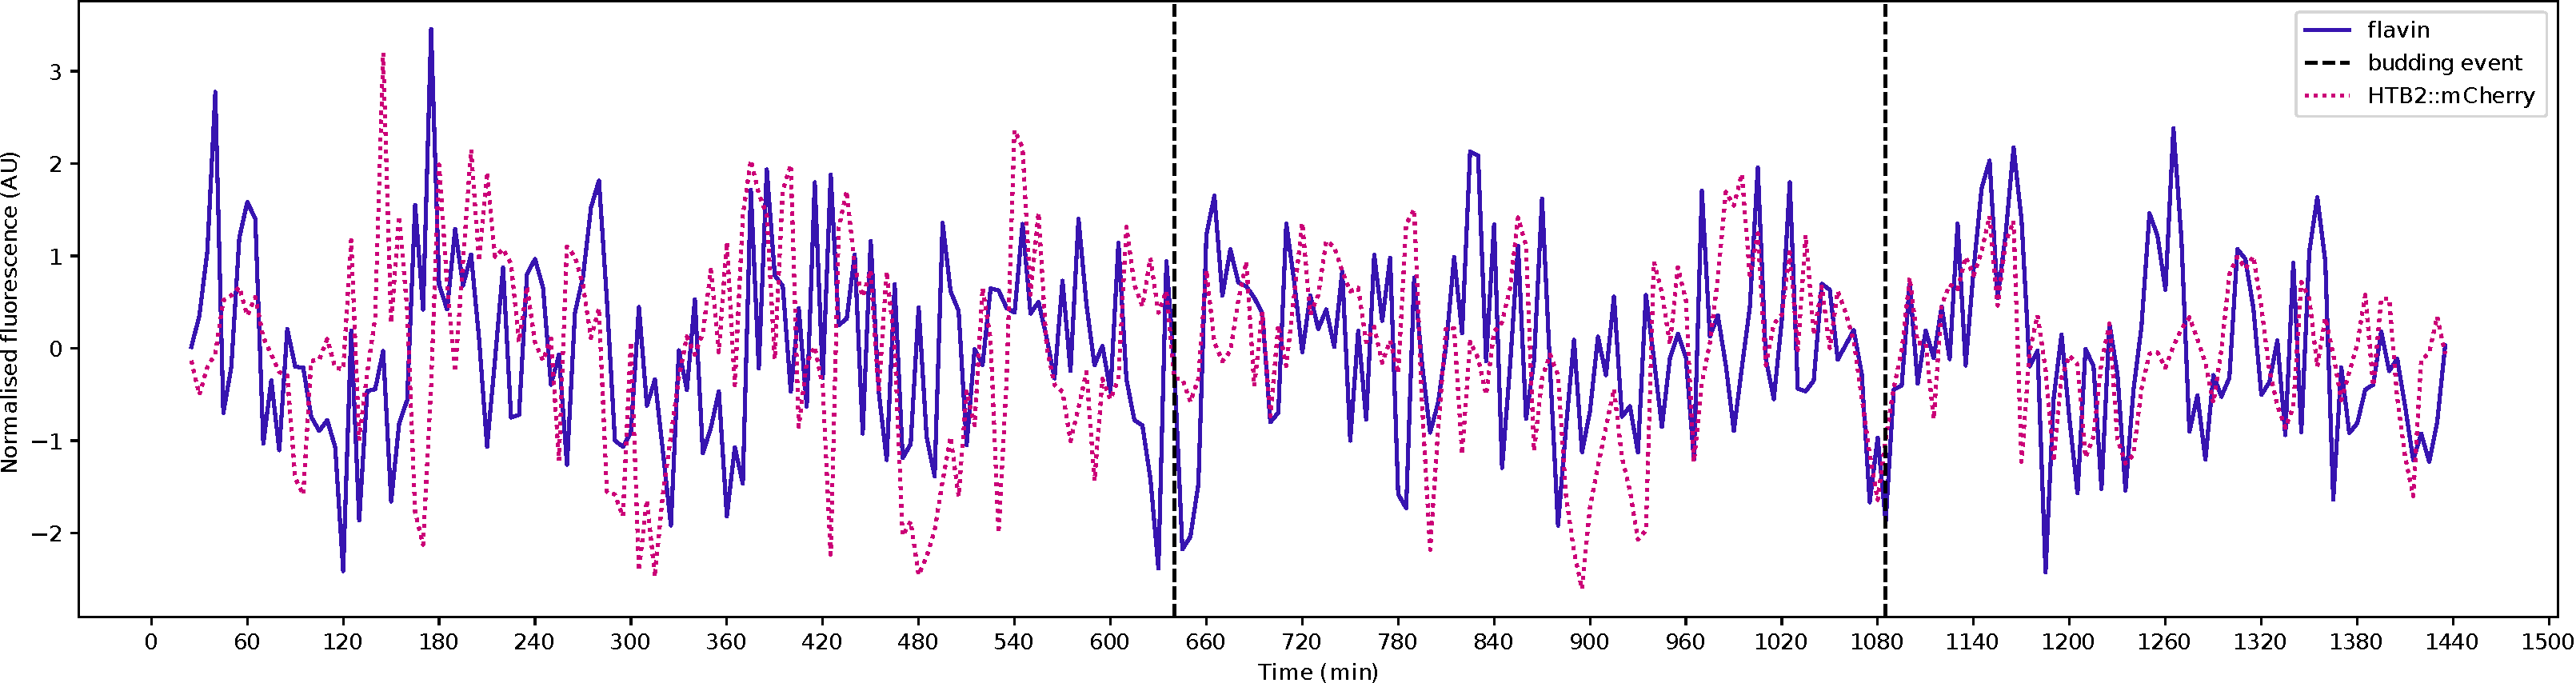
\includegraphics[width=\textwidth]{limiting_single_birth_plot_edit.pdf}
   \caption{
   }
   \label{fig:biology-lowglc-single}
  \end{subfigure}

  \begin{subfigure}[htpb]{0.7\textwidth}
   \centering
   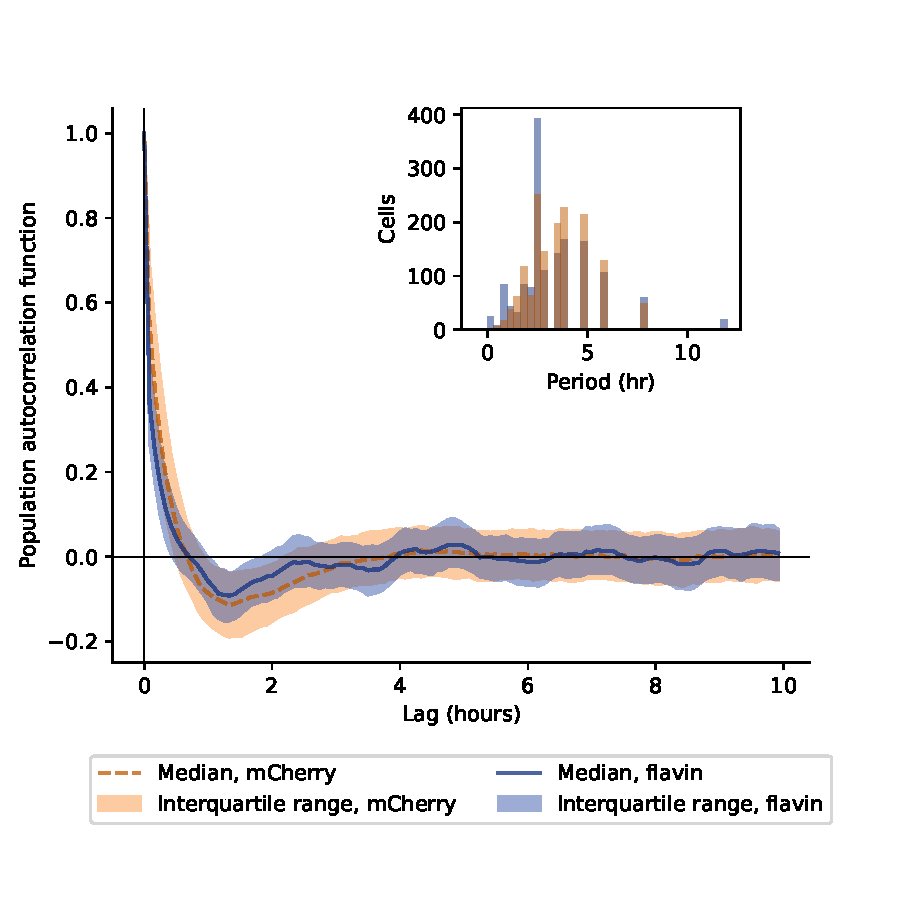
\includegraphics[width=\textwidth]{htb2mCherry_31492_12.pdf}
   \caption{
   }
   \label{fig:biology-lowglc-acf}
  \end{subfigure}
  \caption{
    \textbf{(\ref{fig:biology-lowglc-single})}
    Flavin fluorescence (blue, solid lines) and histone 2B (orange, dotted lines) levels in a single, representative FY4 HTB2::mCherry cell grown in \SI{20}{\gram~\litre^{-1}} pyruvate..
    Vertical lines (black, dashed) indicate budding events.
    \textbf{(\ref{fig:biology-lowglc-acf})}
    Median autocorrelation functions of flavin fluorescence (blue) and histone 2B levels (orange) time series, along with \textit{\textbf{(inset)}} the periods of each oscillator across cells as determined by the frequency with the greatest power in each signal's Fourier spectrum.
    Data are from FY4 HTB2::mCherry cells in \SI{10}{\milli\gram~\litre^{-1}} glucose.
  }
  \label{fig:biology-lowglc}
\end{figure}


% TODO: Plot on same axes, to strengthen comparison between conditions?
\begin{figure}
  \centering
  \begin{subfigure}[htpb]{0.45\textwidth}
   \centering
   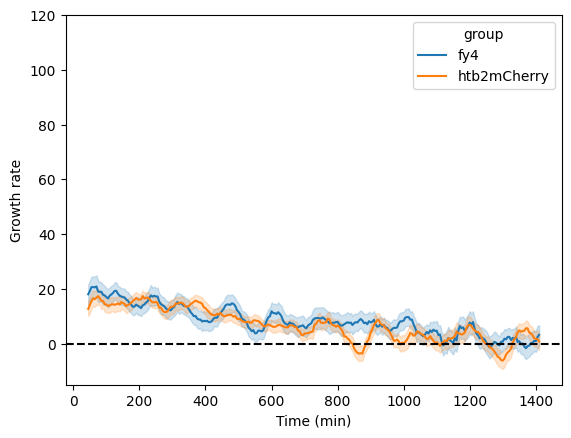
\includegraphics[width=\textwidth]{allstrains_31492_gr}
   \caption{
   }
   \label{fig:biology-lowglc-gr}
  \end{subfigure}%
  \begin{subfigure}[htpb]{0.45\textwidth}
   \centering
   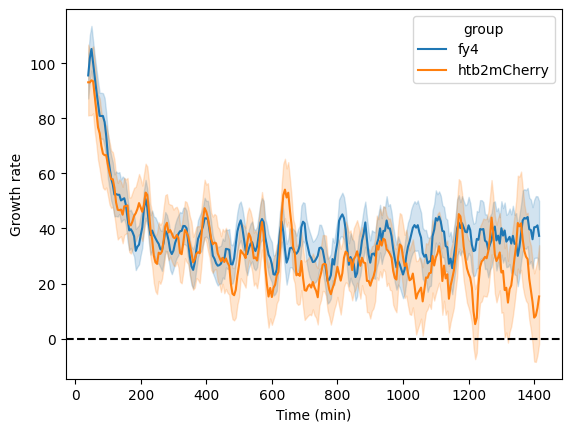
\includegraphics[width=\textwidth]{allstrains_26643_gr}
   \caption{
   }
   \label{fig:biology-highglc-gr}
  \end{subfigure}

  \begin{subfigure}[htpb]{0.45\textwidth}
   \centering
   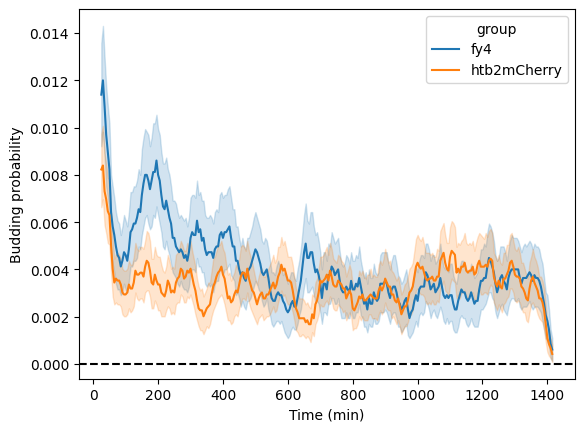
\includegraphics[width=\textwidth]{allstrains_31492_budprob}
   \caption{
   }
   \label{fig:biology-lowglc-budprob}
  \end{subfigure}%
  \begin{subfigure}[htpb]{0.45\textwidth}
   \centering
   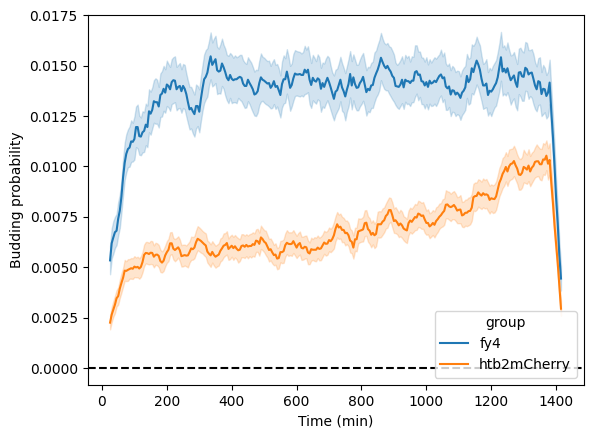
\includegraphics[width=\textwidth]{allstrains_26643_budprob}
   \caption{
   }
   \label{fig:biology-highglc-budprob}
  \end{subfigure}

  \caption{
    Mean growth rate of FY4 (blue) and HTB2::mCherry (orange) strains over time, with 95\% confidence intervals shown (shaded), for \textbf{(\ref{fig:biology-lowglc-gr})} the glucose-limiting condition (\SI{10}{\milli\gram~\litre^{-1}}) and \textbf{(\ref{fig:biology-highglc-gr})} the high glucose condition (\SI{20}{\gram~\litre^{-1}}).
    Similarly, the budding probability of the same strains for \textbf{(\ref{fig:biology-lowglc-budprob})} the glucose-limiting condition and \textbf{(\ref{fig:biology-highglc-budprob})} the high glucose condition.
  }
  \label{fig:biology-lowglc-gr-budprob}
\end{figure}


\begin{figure}
  \centering
  \begin{subfigure}[t]{0.3\textwidth}
   \centering
   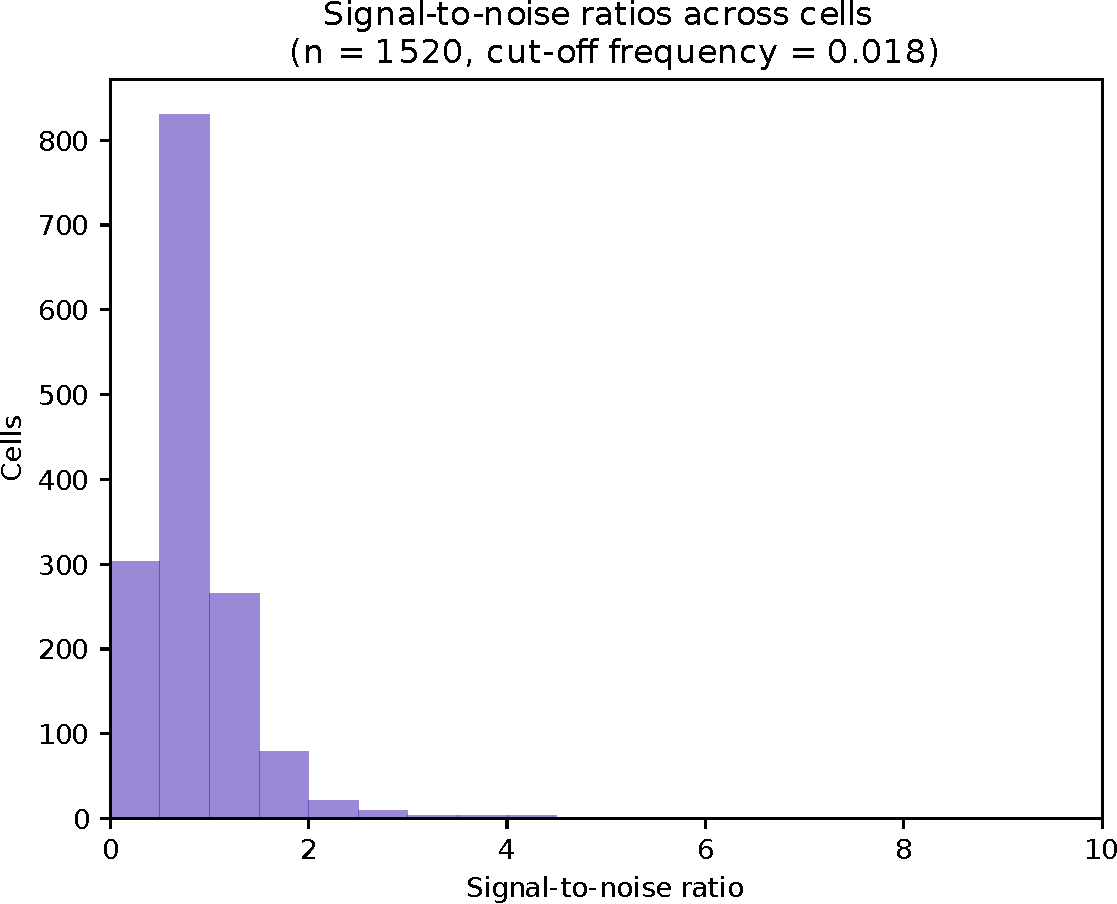
\includegraphics[width=\textwidth]{limiting_snr_edit}
   \caption{
   }
   \label{fig:biology-lowglc-snr}
  \end{subfigure}%
  \begin{subfigure}[t]{0.3\textwidth}
   \centering
   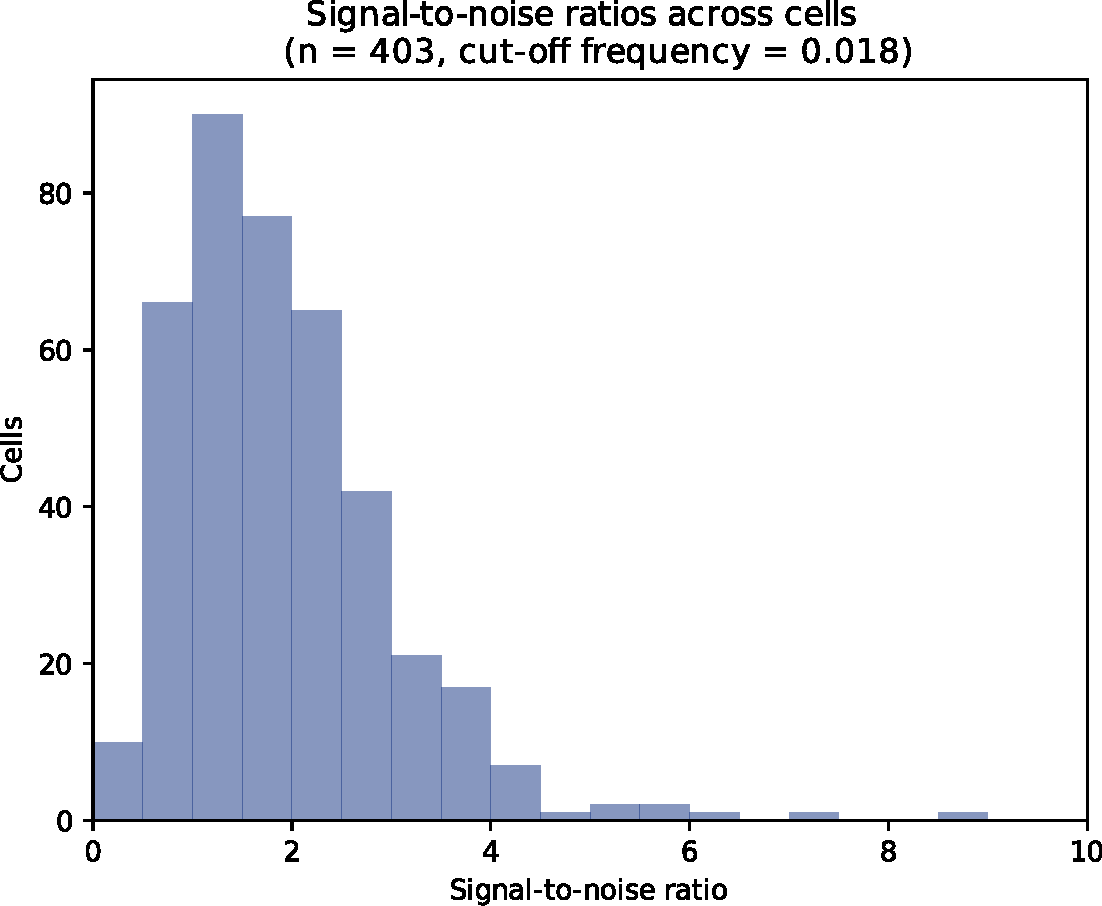
\includegraphics[width=\textwidth]{pyruvate_snr_edit}
   \caption{
   }
   \label{fig:biology-pyruvate-snr}
  \end{subfigure}%
  \begin{subfigure}[t]{0.3\textwidth}
   \centering
   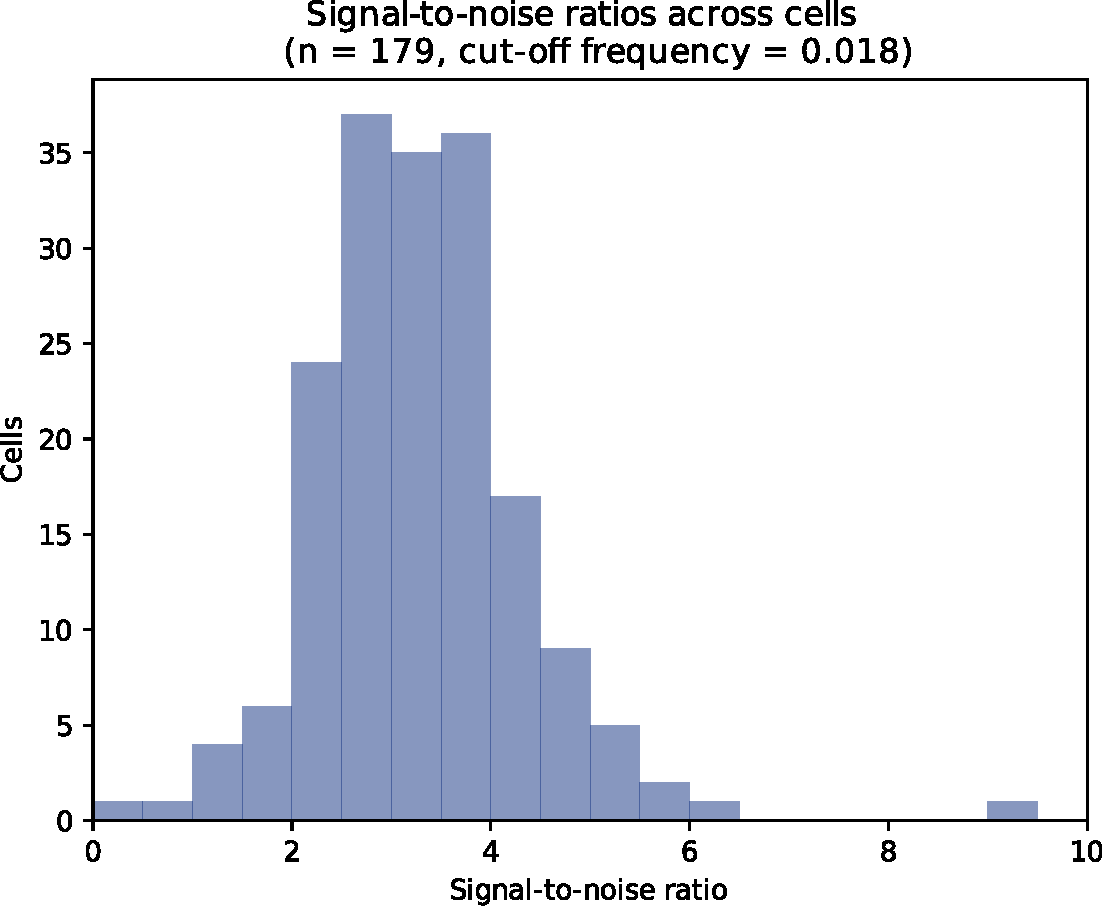
\includegraphics[width=\textwidth]{glucose_snr_edit}
   \caption{
   }
   \label{fig:biology-highglc-snr}
  \end{subfigure}

  \caption{
    Distribution of signal-to-noise ratios of flavin signals from cells in
    \textbf{(\ref{fig:biology-lowglc-snr})}
    \SI{10}{\milli\gram~\litre^{-1}} glucose,
    \textbf{(\ref{fig:biology-pyruvate-snr})}
    \SI{20}{\gram~\litre^{-1}} pyruvate, and
    \textbf{(\ref{fig:biology-highglc-snr})}
    \SI{20}{\gram~\litre^{-1}} glucose.
  }
  \label{fig:biology-compare-snr}
\end{figure}


Fig.\ \ref{fig:biology-lowglc} shows that FY4 HTB2::mCherry cells showed longer metabolic cycles when grown in minimal media supplemented with \SI{10}{\milli\gram~\litre^{-1}} glucose.
Additionally, Fig.\ ~\ref{fig:biology-lowglc-gr-budprob} shows that the growth rate and the budding probability of cells on limiting glucose is lower than on high glucose (\SI{20}{\gram~\litre^{-1}}).

Furthermore, Fig.\ \ref{fig:biology-compare-snr} shows that the amplitude of the flavin oscillations in this limiting-glucose condition was low relative to other conditions, as evidenced by the lower signal-to-noise ratios (INSERT: statistical tests to reject the null hypothesis that the distribution of SNRs are the same between the three nutrient conditions.).

Finally, Fig.\ \ref{fig:biology-lowglc-acf} shows that the metabolic cycle and the cell division cycle lost synchrony in limiting glucose.
This was evidenced by a \SI{2.5}{\hour} average metabolic cycle, though not robust, but an absence of consistent oscillations in mCherry intensity.
This decoupling could be explained by a lack of cell division cycle events.

% In contrast to 20 g/L glucose in which metabolic cycles were asynchronous, in these conditions there is some degree of metabolic cycle synchrony between cells. \textbf{(add figures)}

% TODO: How are these linked to Papagiannakis et al.?  Am I getting the same conclusions?  Also -- space to discuss the 10-hour oscillations in chemostats in slow dilution rates.


%\section[Potassium-deficient media]{Do single-cell flavin traces recapitulate dissolved-oxygen YMCs in chemostats? -- potassium-deficient media}
\section{Metabolic cycles persist in potassium-deficient media}
\label{sec:biology-potassium_deficient}

To address whether single-cell flavin traces from my microfluidics experiments recapitulate dissolved-oxygen yeast metabolic cycles in chemostats, I replicated conditions of chemostat-based studies that demonstrated nutrient or genetic perturbations that severely affected the metabolic cycle.
These include potassium deficiency along with the zwf1$\Delta$ and tsa1$\Delta$ tsa2$\Delta$ deletions.
This is important in showing that the single-cell metabolic cycle and the chemostat metabolic cycle are the same cycle, or to prove otherwise.
Chemostat experiments obscure the behaviour of individual cells, and
my single-cell microfluidics experiments could provide a bottom-up explanation of high-level observations of the metabolic cycle in the chemostat; for example, whether the cellular behaviour of the yeast metabolic cycle explains the changes in dissolved-oxygen oscillations.


\begin{figure}
  \centering
  \begin{subfigure}[htpb]{1.0\textwidth}
   \centering
   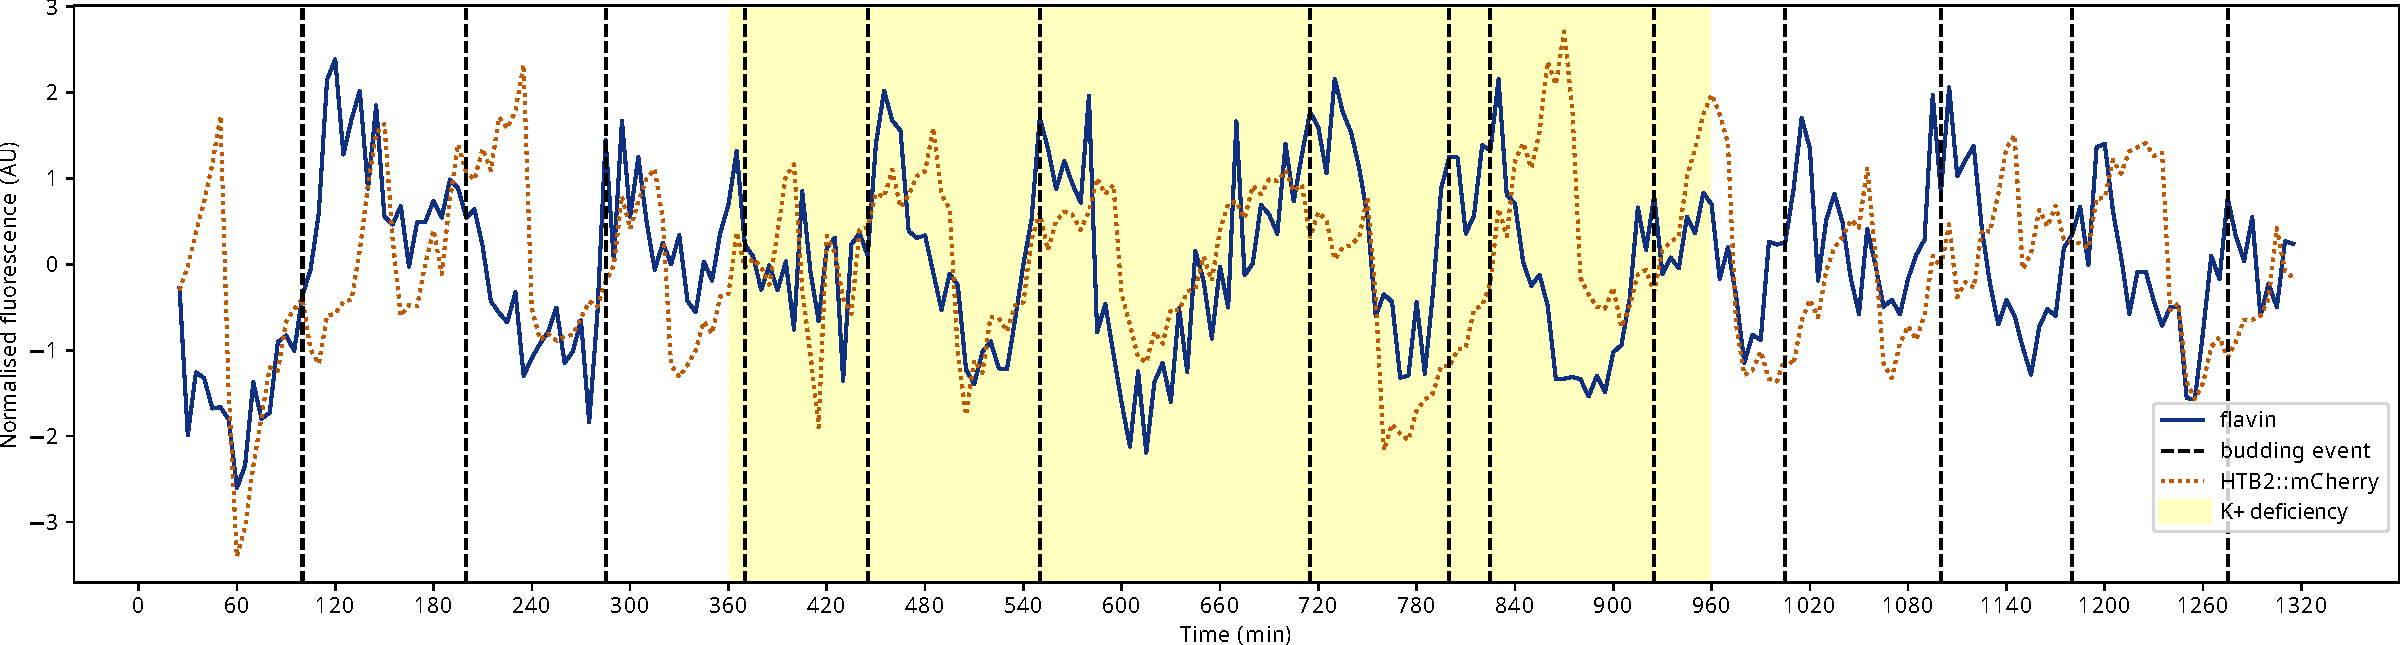
\includegraphics[width=\textwidth]{htb2mCherry_613_plots_single_htb2mCherry012_90_2_adapted.pdf}
   \caption{
   }
   \label{fig:biology-kdeficient-single}
  \end{subfigure}

  \begin{subfigure}[htpb]{0.7\textwidth}
   \centering
   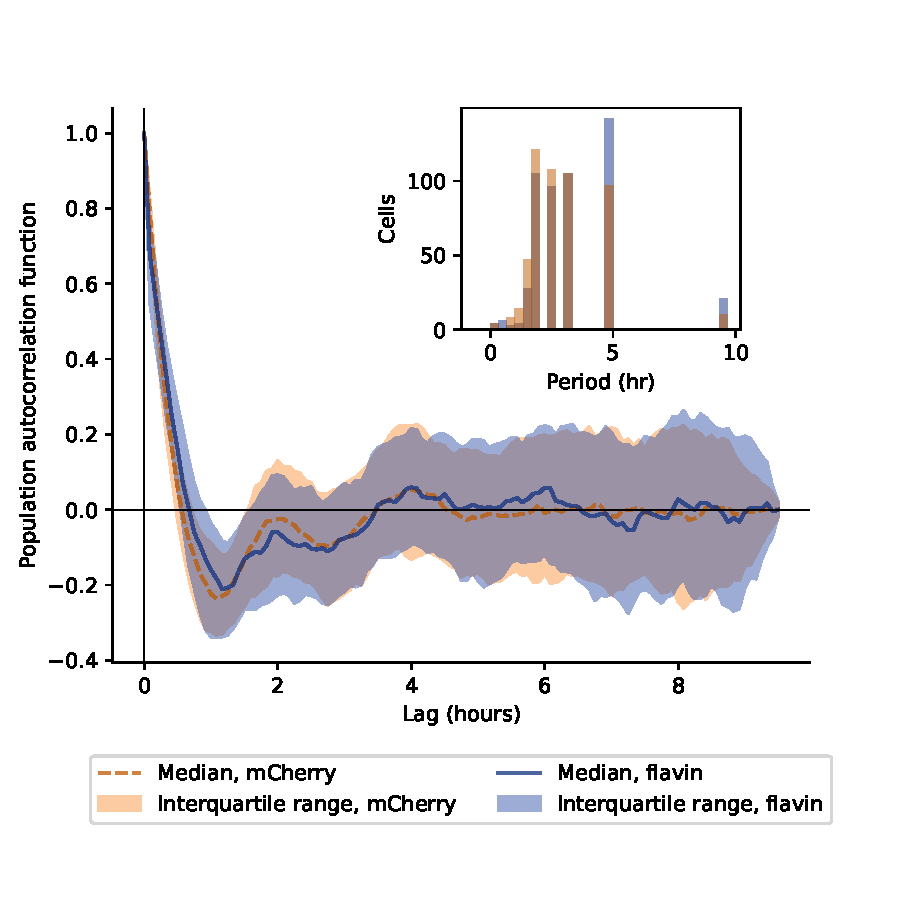
\includegraphics[width=\textwidth]{htb2mCherry_613_12.pdf}
   \caption{
   }
   \label{fig:biology-kdeficient-acf}
  \end{subfigure}

  \caption{
    \textbf{(\ref{fig:biology-kdeficient-single})}
    Flavin fluorescence (blue, solid lines) and histone 2B (orange, dotted lines) levels in a single, representative FY4 HTB2::mCherry cell.
    Vertical lines (black, dashed) indicate budding events.
    Shading indicates the potassium-deficient period.
    \textbf{(\ref{fig:biology-kdeficient-acf})}
    Median autocorrelation functions of flavin fluorescence (blue) and histone 2B levels (orange) time series, along with \textit{\textbf{(inset)}} the periods of each oscillator across cells as determined by the frequency with the greatest power in each signal's Fourier spectrum.
    Data are from FY4 and HTB2::mCherry cells, subject to normal medium for \SI{6}{\hour} before being abruptly switched to potassium-deficient medium for \SI{10}{\hour} and then resumed to normal medium for \SI{6}{\hour}.
  }
  \label{fig:biology-kdeficient}
\end{figure}


\begin{figure}
  \centering
  \begin{subfigure}[htpb]{0.45\textwidth}
   \centering
   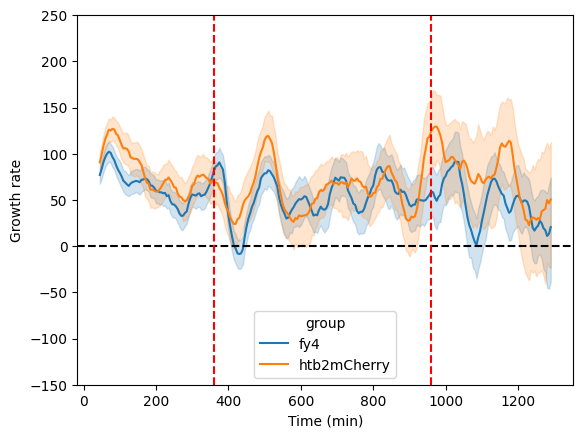
\includegraphics[width=\textwidth]{allstrains_613_gr}
   \caption{
   }
   \label{fig:biology-kdeficient-gr}
  \end{subfigure}%
  \begin{subfigure}[htpb]{0.45\textwidth}
   \centering
   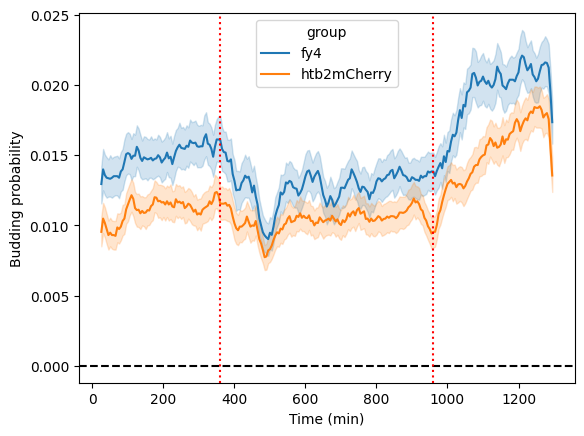
\includegraphics[width=\textwidth]{allstrains_613_budprob}
   \caption{
   }
   \label{fig:biology-kdeficient-budprob}
  \end{subfigure}

  \caption{
    \textbf{(\ref{fig:biology-kdeficient-gr})}
    Mean growth rate and
    \textbf{(\ref{fig:biology-kdeficient-budprob})}
    budding probability of FY4 (blue) and HTB2::mCherry (orange) strains over time during the potassium-deficient experiment, with 95\% confidence intervals shown (shaded).
    Vertical lines (red) show changes in nutrient media.
  }
  \label{fig:biology-kdeficient-gr-budprob}
\end{figure}


To test whether potassium deficiency eliminates metabolic cycles, Fig.\ \ref{fig:biology-kdeficient-single} shows that FY4 HTB2::mCherry cells retained synchronised metabolic cycles and cell division cycles when cells were abruptly switched from potassium-containing to potassium-deficient minimal medium (both media supplemented with \SI{20}{\gram~\litre^{-1}} as a carbon source).
Such cycles were longer and generated less reliably as in the normal growth medium (Fig.\ \ref{fig:biology-kdeficient-acf}).
In addition, to test whether potassium deficiency affected cell growth and division, Fig.\ \ref{fig:biology-kdeficient-gr} recovered soon after a sharp decrease upon the abrupt switch to the potassium-deficient median.
Fig.\ \ref{fig:biology-kdeficient-budprob} further shows that the budding probability only showed a slight drop during potassium-deficiency, in contrast to a near-zero drop under glucose starvation (Fig.\ \ref{fig:biology-starvation-budprob}).

\begin{figure}
  \centering
  
\includegraphics[width=0.7\textwidth]{placeholder01.pdf}
  \caption{
    Insert caption here.
    This is the heatmap/histogram for the potassium-deficient experiment.
  }
  \label{fig:biology-kdeficient-histogram}
\end{figure}

(INSERT 1--2 PARAGRAPHS OF INTERPRETATION OF NEW HEATMAP)


\begin{figure}
  \centering
  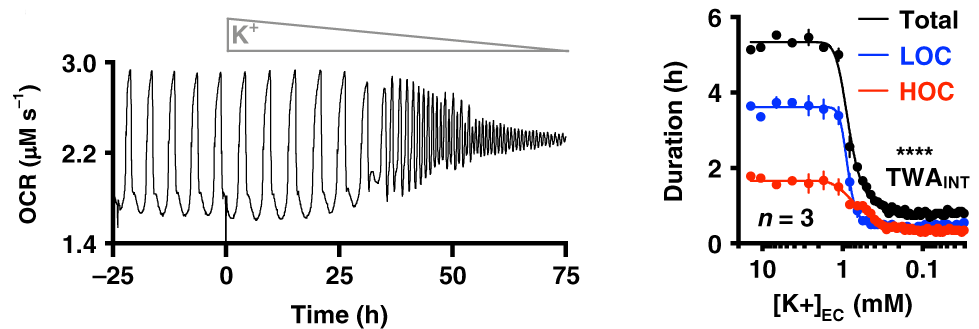
\includegraphics[width=0.7\textwidth]{oneillEukaryoticCellBiology2020_4_adapted.png}
  \caption{
    Decreasing extracellular potassium (\ce{K+}) concentration shortens, then under \SI{1}{\milli\molar}, destroys metabolic oscillations in the chemostat.
    Adapted from \textcite{oneillEukaryoticCellBiology2020}.
  }
  \label{fig:biology-kdeficient-oneill}
\end{figure}

Results thus suggest that even though there is an initial response to potassium depletion, cells resume growth, division, and generation of metabolic cycles soon after.
My observations show that the metabolic cycle still occur in a drastically changed nutrient condition.
This is in contrast to \textcite{oneillEukaryoticCellBiology2020}, which suggested that as potassium is graduate replaced with sodium in chemostat culture media, the amplitude of dissolved-oxygen oscillations decrease until they disappear altogether (Fig.\ \ref{fig:biology-kdeficient-oneill}).
However, my observations also warrant a model to reconcile the apparent differences between the chemostat and single-cell investigations.


%\section[Deletion strains]{Do single-cell flavin traces recapitulate dissolved-oxygen YMCs in chemostats? -- deletion strains}
\section{Metabolic cycles in deletion strains}
\label{sec:biology-deletions}

% \item swe1$\Delta$: gene responsible for CDC processes (another biological rhythm) e.g. DNA repair.  Deletion shown to affect CDC-YMC coupling.
% \item rim11$\Delta$: gene involved in circadian rhythm (another biological rhythm).  Deletion strain shown to have shorter YMCs.

To continue the investigation of whether single-cell flavin-based metabolic cycles recapitulate dissolved-oxygen metabolic cycles, I investigated the zwf1$\Delta$ and tsa1$\Delta$ tsa2$\Delta$ deletion strains.
Deletion strains could give mechanistic insight on the YMC.


% TODO: Add single time series??  I've shown them for all the experiments so far, I just realised.
\begin{figure}
  \centering
  \begin{subfigure}[t]{1.0\textwidth}
   \centering
   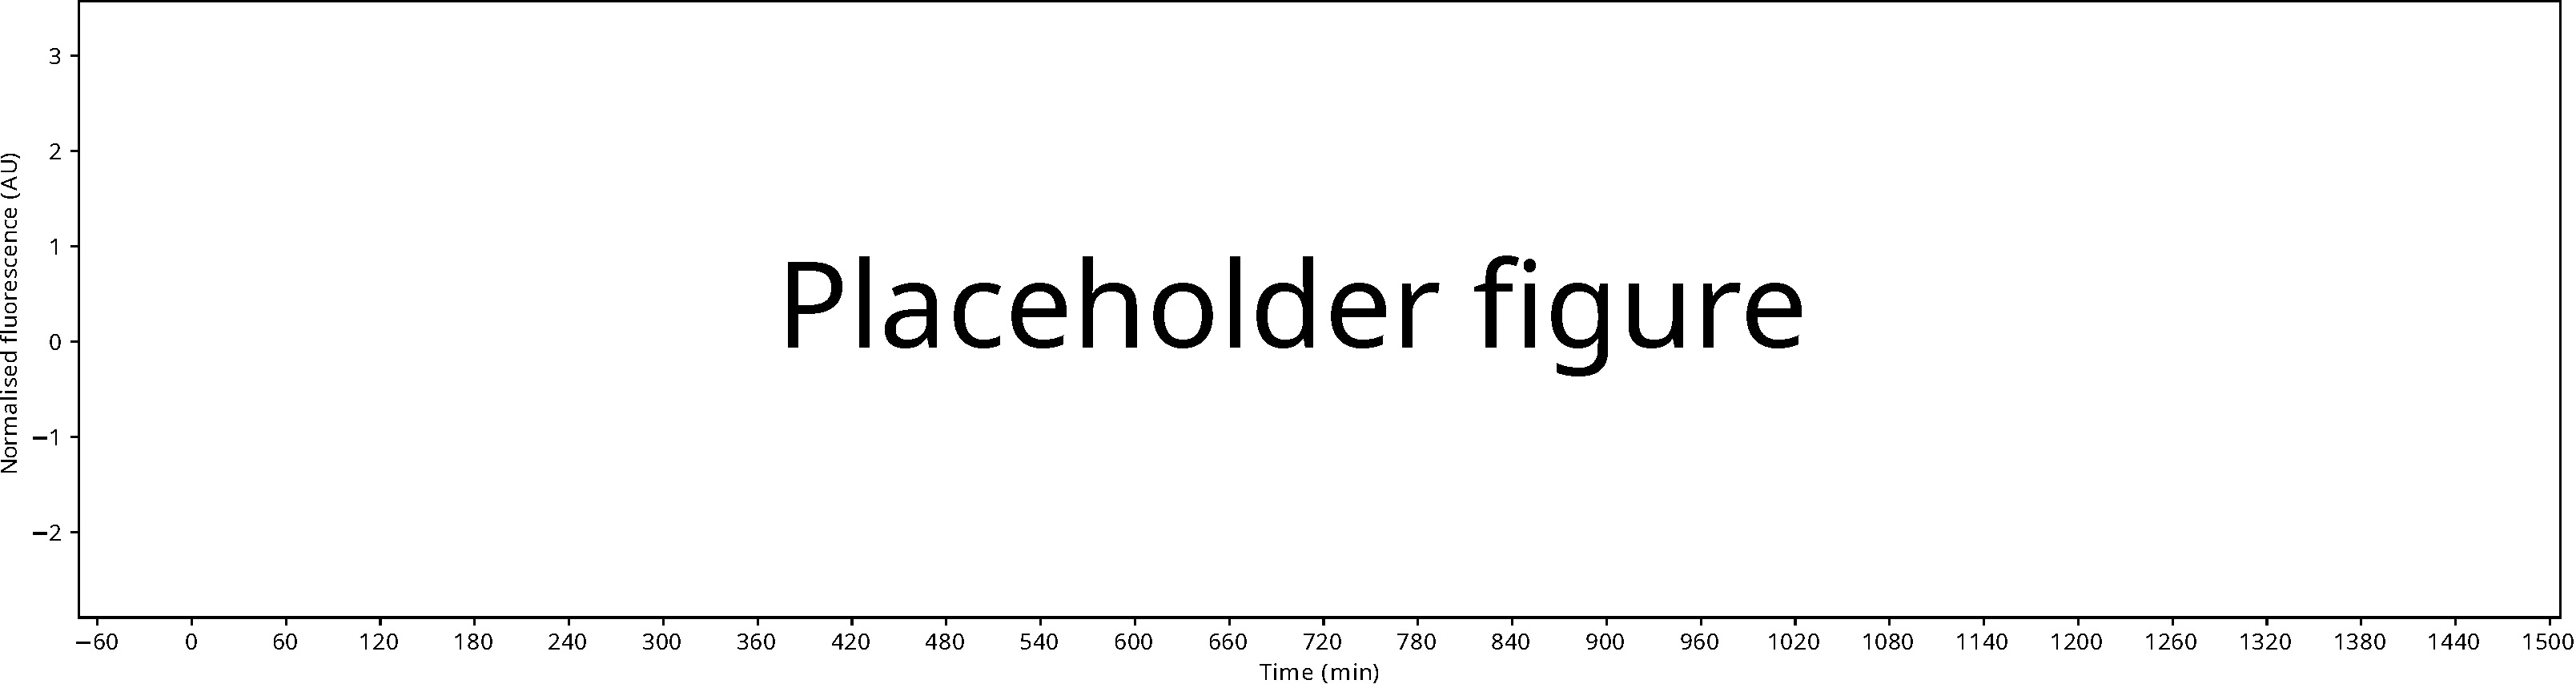
\includegraphics[width=\textwidth]{placeholder02.pdf}
   \caption{
   }
   \label{fig:biology-zwf1-single}
  \end{subfigure}

  \begin{subfigure}[t]{0.45\textwidth}
   \centering
   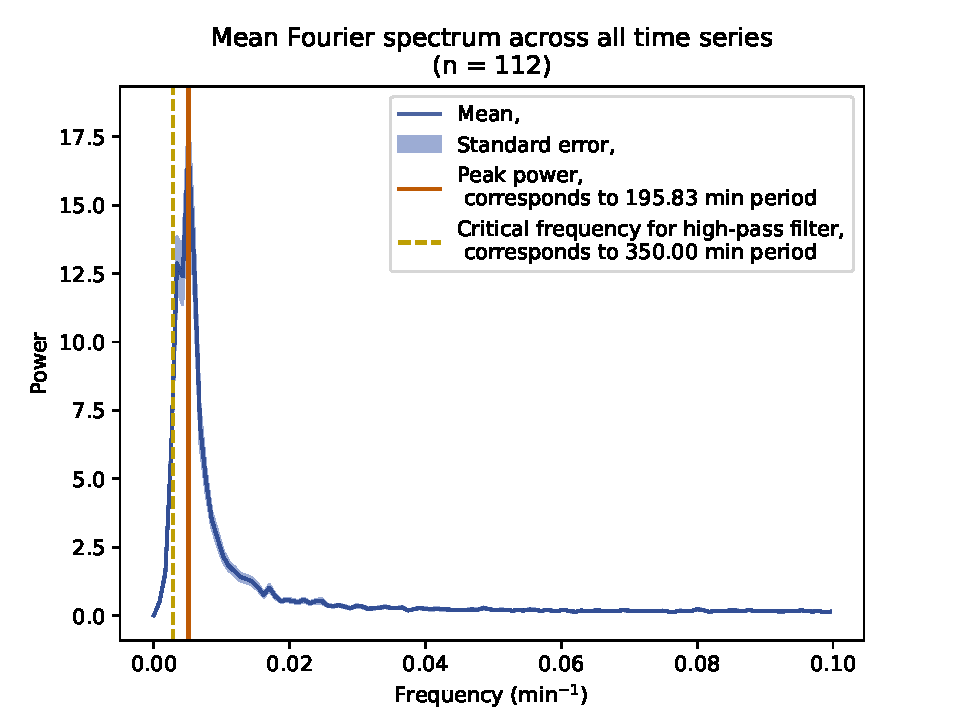
\includegraphics[width=\textwidth]{zwf1egf_409_13.pdf}
   \caption{
   }
   \label{fig:biology-zwf1-fourier}
  \end{subfigure}%
  \begin{subfigure}[t]{0.45\textwidth}
   \centering
   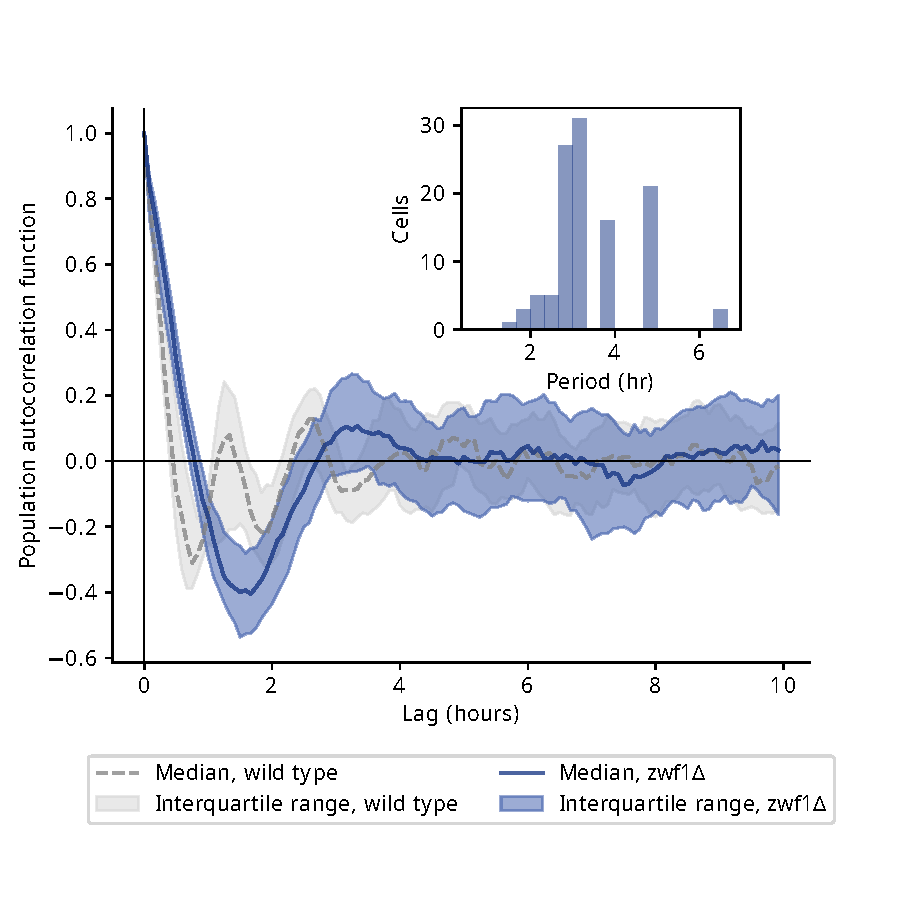
\includegraphics[width=\textwidth]{zwf1egf_409_12.pdf}
   \caption{
   }
   \label{fig:biology-zwf1-acf}
  \end{subfigure}

  \begin{subfigure}[t]{0.45\textwidth}
   \centering
   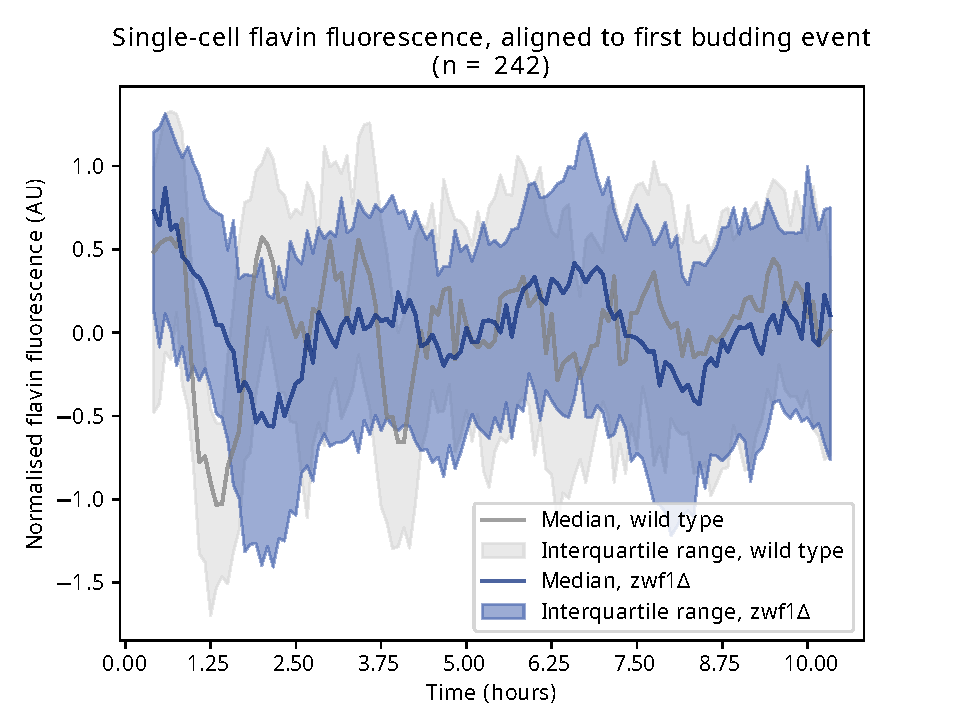
\includegraphics[width=\textwidth]{zwf1egf_409_6.pdf}
   \caption{
   }
   \label{fig:biology-zwf1-median}
  \end{subfigure}%
  \begin{subfigure}[t]{0.45\textwidth}
   \centering
   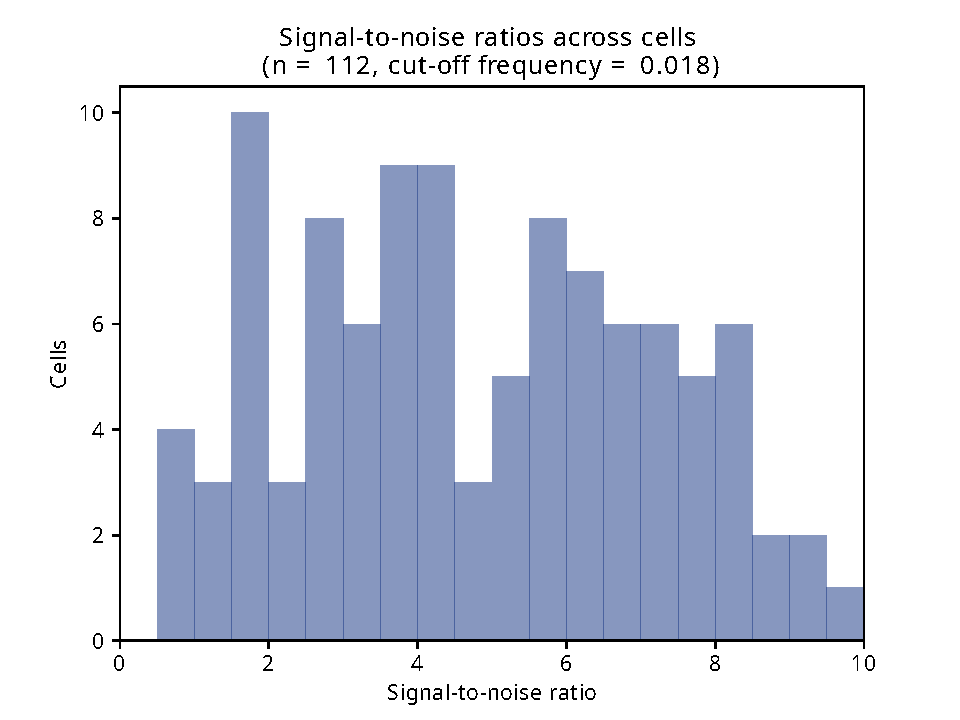
\includegraphics[width=\textwidth]{zwf1egf_409_10.pdf}
   \caption{
   }
   \label{fig:biology-zwf1-snr}
  \end{subfigure}%

  \caption{
    \textbf{(\ref{fig:biology-zwf1-single})}
    Flavin fluorescence (blue, solid lines) levels in a single, representative zwf1$\Delta$ cell.
    Vertical lines (black, dashed) indicate budding events.
    \textbf{(\ref{fig:biology-zwf1-fourier})}
    Mean Fourier spectrum of flavin fluorescence across cells.
    \textbf{(\ref{fig:biology-zwf1-acf})}
    Median autocorrelation function of flavin fluorescence time series, along with \textit{\textbf{(inset)}} the periods of each oscillator across cells as determined by the frequency with the greatest power in each signal's Fourier spectrum.
    \textbf{(\ref{fig:biology-zwf1-median})}
    Median flavin fluorescence signal across cells, aligned to first budding event.
    \textbf{(\ref{fig:biology-zwf1-snr})}
    Distribution of signal-to-noise ratios of flavin signals from cells.
    Data are from zwf1$\Delta$ (BY4741) cells in \SI{10}{\gram~\litre^{-1}} glucose.
  }
  \label{fig:biology-zwf1}
\end{figure}


To investigate whether the zwf1$\Delta$ strain shows abolition of the metabolic cycle in single-cell microfluidics, I used a zwf1$\Delta$ strain with the BY4741 background.
Chemostat-based studies suggest that in the zwf1$\Delta$ strain, metabolic cycles are abolished but with little change in growth rate \parencite{tuCyclicChangesMetabolic2007}.
% Move to methods?
Cells were pre-cultured in \SI{20}{\gram~\litre^{-1}} pyruvate over \SI{48}{\hour} and then cultured in \SI{10}{\gram~\litre^{-1}} glucose in the microfluidic device as higher glucose concentrations disfavour growth in this strain.
As the strain had an auxotrophic background, the required nutrient supplements were also added.
%
Figure~\ref{fig:biology-zwf1} shows that the zwf$\Delta$ showed oscillations of approximately \SI{3}{\hour}, but with low robustness and a wide distribution of signal-to-noise ratios, while the reference BY4741 strain showed robust flavin oscillations of approximately \SI{1.5}{\hour}.
These results conflict with the results from the chemostat-based study \parencite{tuCyclicChangesMetabolic2007} that suggests that metabolic cycles are abolished in this strain.


\begin{figure}
  \centering
  \begin{subfigure}[t]{1.0\textwidth}
   \centering
   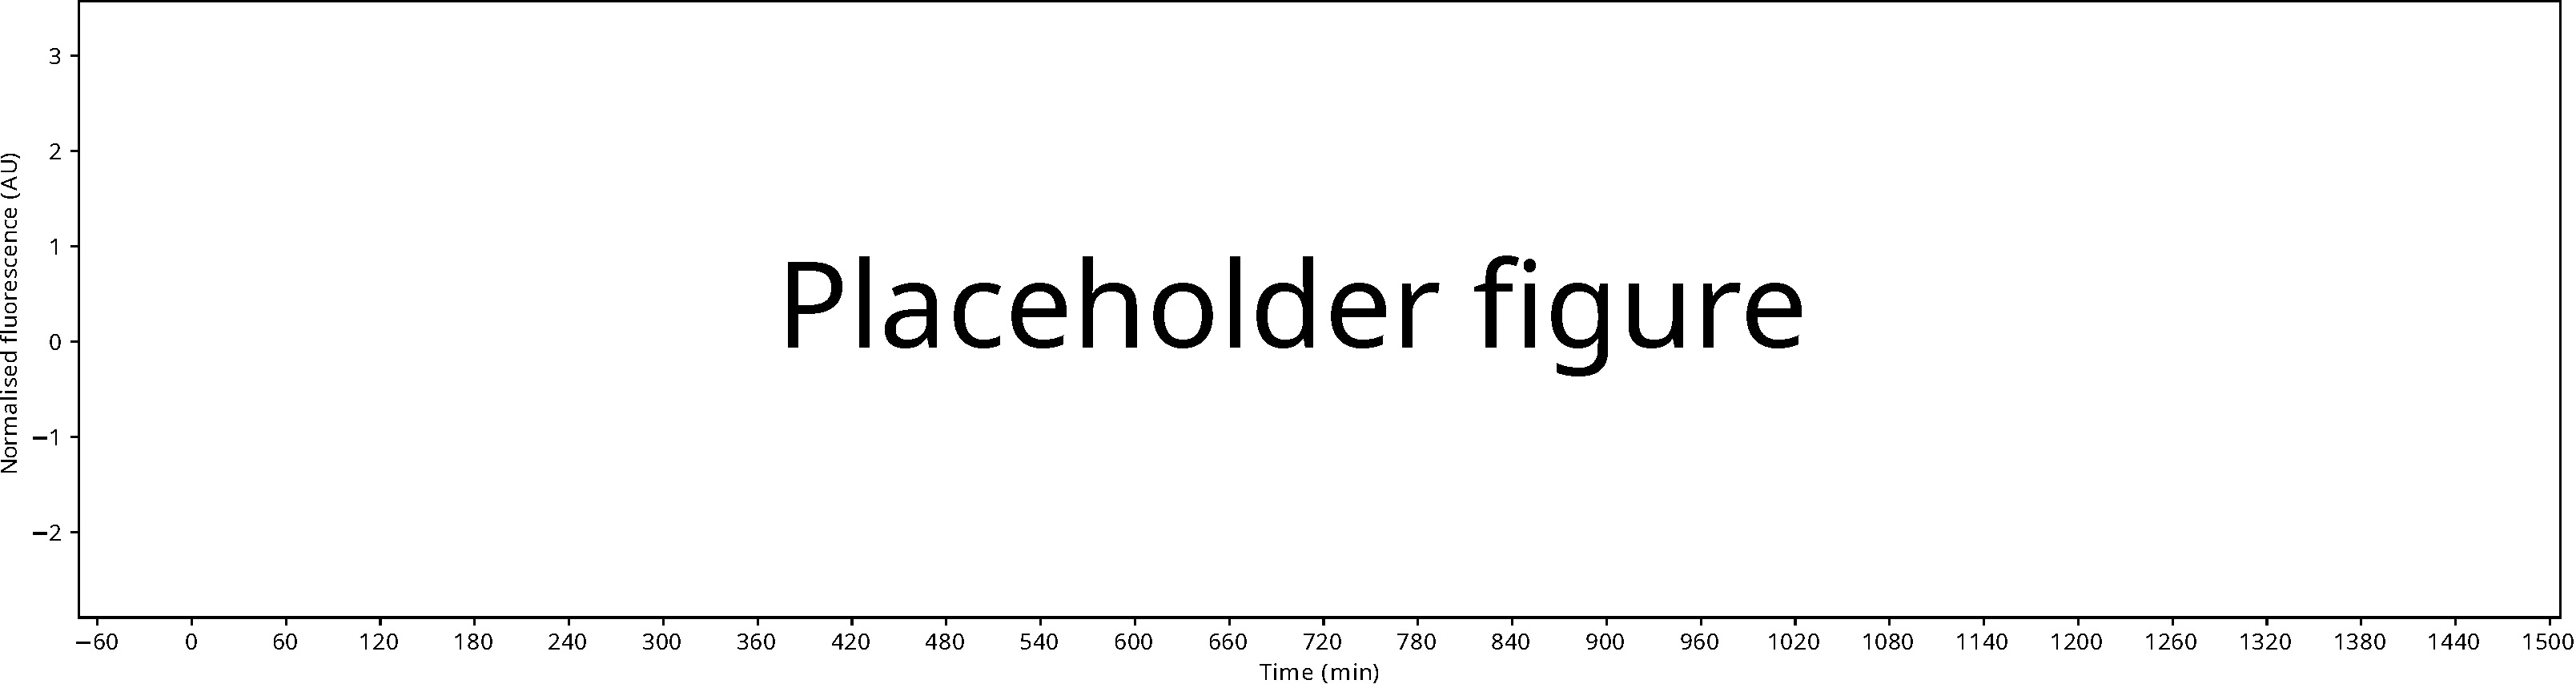
\includegraphics[width=\textwidth]{placeholder02.pdf}
   \caption{
   }
   \label{fig:biology-tsa1tsa2-single}
  \end{subfigure}

  \begin{subfigure}[t]{0.45\textwidth}
   \centering
   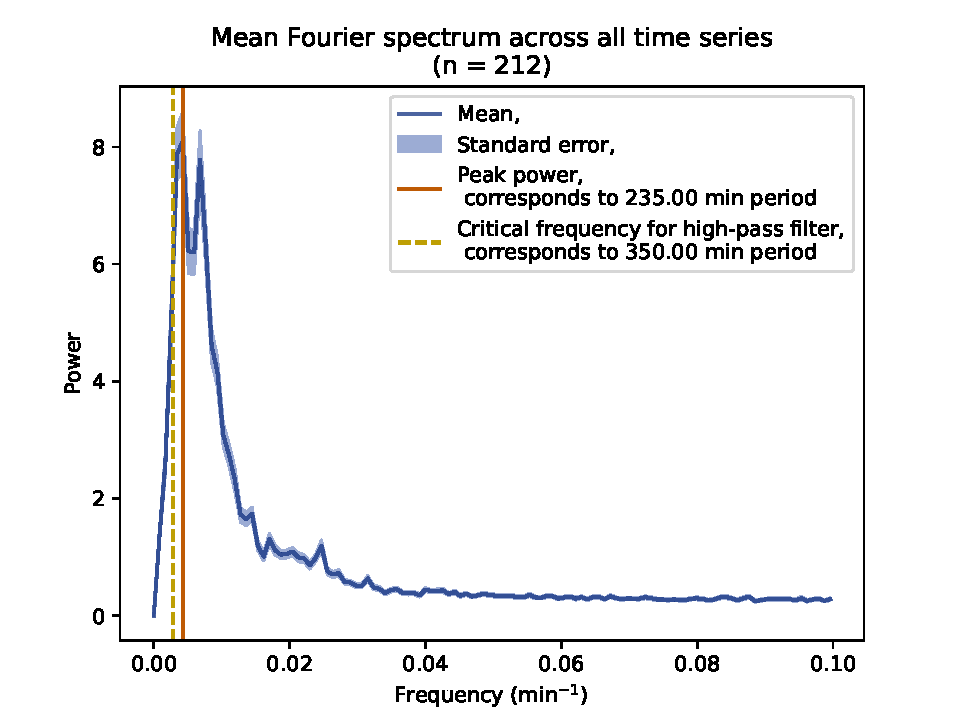
\includegraphics[width=\textwidth]{tsa1tsa2morgan_1649_13.pdf}
   \caption{
   }
   \label{fig:biology-tsa1tsa2-fourier}
  \end{subfigure}%
  \begin{subfigure}[t]{0.45\textwidth}
   \centering
   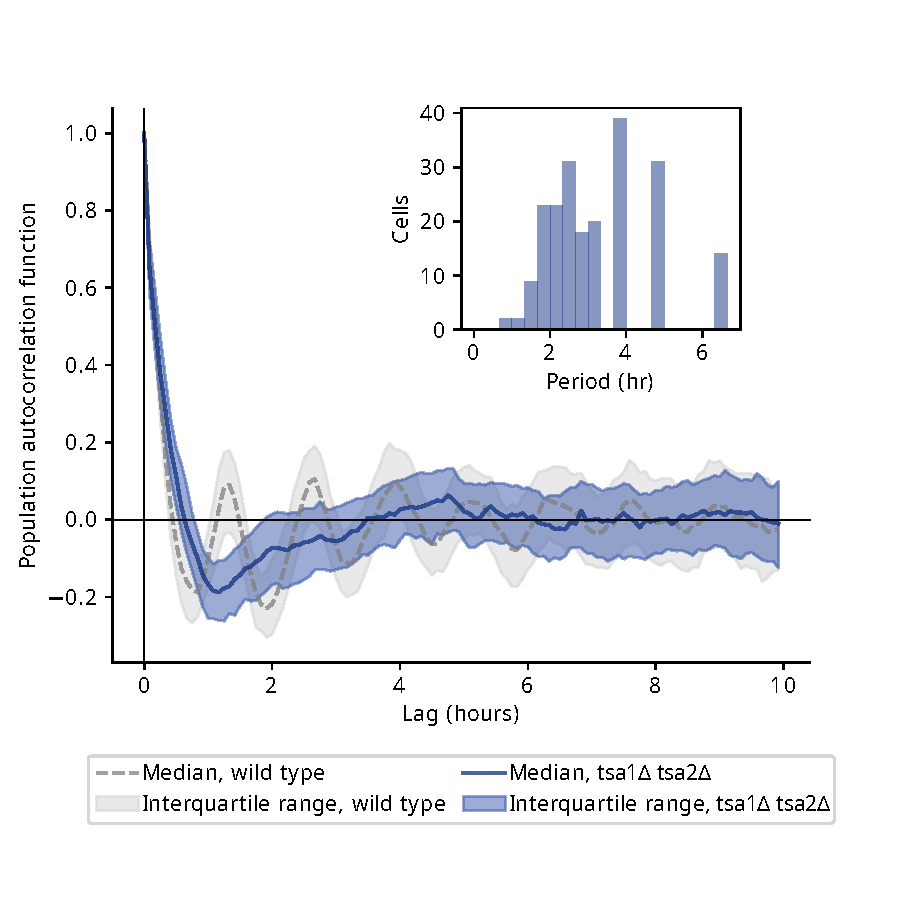
\includegraphics[width=\textwidth]{tsa1tsa2morgan_1649_12.pdf}
   \caption{
   }
   \label{fig:biology-tsa1tsa2-acf}
  \end{subfigure}

  \begin{subfigure}[t]{0.45\textwidth}
   \centering
   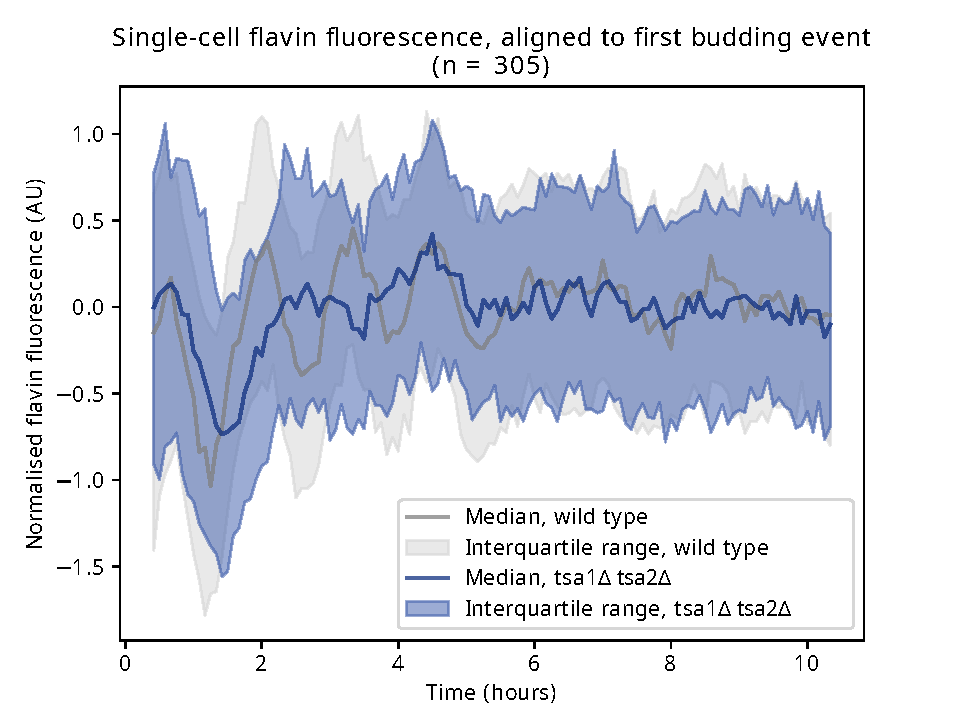
\includegraphics[width=\textwidth]{tsa1tsa2morgan_1649_6.pdf}
   \caption{
   }
   \label{fig:biology-tsa1tsa2-median}
  \end{subfigure}%
  \begin{subfigure}[t]{0.45\textwidth}
   \centering
   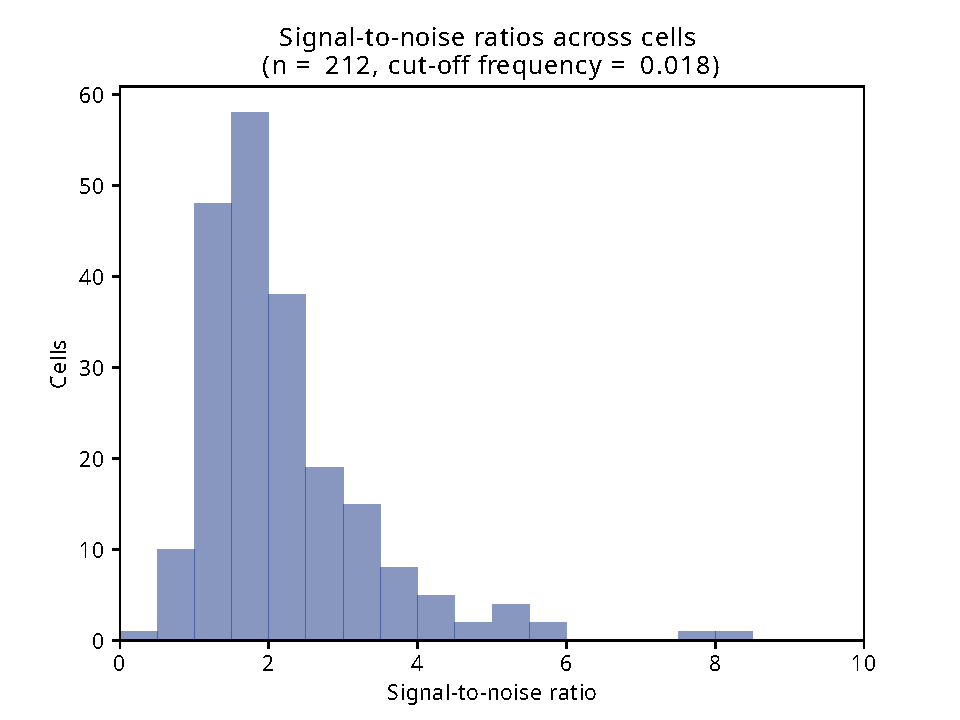
\includegraphics[width=\textwidth]{tsa1tsa2morgan_1649_10.pdf}
   \caption{
   }
   \label{fig:biology-tsa1tsa2-snr}
  \end{subfigure}

  \caption{
    \textbf{(\ref{fig:biology-tsa1tsa2-single})}
    Flavin fluorescence (blue, solid lines) levels in a single, representative tsa1$\Delta$ tsa2$\Delta$cell.
    Vertical lines (black, dashed) indicate budding events.
    \textbf{(\ref{fig:biology-tsa1tsa2-fourier})}
    Mean Fourier spectrum of flavin fluorescence across cells.
    \textbf{(\ref{fig:biology-tsa1tsa2-acf})}
    Median autocorrelation function of flavin fluorescence time series, along with \textit{\textbf{(inset)}} the periods of each oscillator across cells as determined by the frequency with the greatest power in each signal's Fourier spectrum.
    \textbf{(\ref{fig:biology-tsa1tsa2-median})}
    Median flavin fluorescence signal across cells, aligned to first budding event.
    \textbf{(\ref{fig:biology-tsa1tsa2-snr})}
    Distribution of signal-to-noise ratios of flavin signals from cells.
    Data are from tsa1$\Delta$ tsa2$\Delta$ (BY4742) cells in \SI{10}{\gram~\litre^{-1}} glucose.
  }
  \label{fig:biology-tsa1tsa2}
\end{figure}


To investigate whether the tsa1$\Delta$ tsa2$\Delta$ strain shows metabolic oscillations of a different waveform in single-cell microfluidics, I used a tsa1$\Delta$ tsa2$\Delta$ strain with the BY4742 background.
Chemostat-based studies suggest that in the tsa1$\Delta$ tsa2$\Delta$ strain, metabolic cycles are shorter and exhibit an M-shaped dissolved oscillation trace due to an additional dip of oxygen consumption in the reductive-charging phase \parencite{caustonMetabolicCyclesYeast2015}.
% Move to methods?
To be consistent with zwf1$\Delta$, cells were pre-cultured and cultured in the same conditions, but with the appropriate supplements for the auxotrophy of BY4742.
%
% Is this because of a wide variety of oscillation frequencies?  Look at the FFT inset, or do additional investigations.

Fig.\ \ref{fig:biology-tsa1tsa2} suggests that the auxotrophic tsa1$\Delta$ tsa2$\Delta$ strain does not reliably generate metabolic cycles.
The median fluorescence signal aligned by first budding event (Fig.\ \ref{fig:biology-tsa1tsa2-median}) and the mean Fourier spectrum (Fig.\ \ref{fig:biology-tsa1tsa2-fourier}) suggest that a \SI{3}{\hour} oscillation is prominent in the population;
however, the median autocorrelation function (Fig.\ \ref{fig:biology-tsa1tsa2-acf}) suggests that the oscillations are not at a consistent frequency across the population, in contrast to the BY4742 wild-type that shows robust \SI{1.5}{\hour} oscillations.
Fig.\ \ref{fig:biology-tsa1tsa2-snr} additionally suggests that the loss of robust oscillations is not due to lower amplitudes or lower qualities of oscillations, as evidenced by signal-to-noise ratios comparable to the FY4 strain cultured in pyruvate (Fig.\ \ref{fig:biology-pyruvate-snr}; ADD STATISTICAL TEST HERE).

Taken together, there are striking discrepancies between the metabolic cycle observed as dissolved oxygen oscillations from the chemostat and the metabolic cycle observed as flavin autofluorescence oscillations in single-cell conditions in the zwf1$\Delta$ and tsa1$\Delta$ tsa2$\Delta$ deletion strains.
These discrepancies warrant further explanation.


\section{Discussion}
\label{sec:biology-discussion}

\subsection{Interpretation of results}
\label{subsec:biology-discussion-interpretation}

This chapter confirms the presence of flavin-based single-cell metabolic cycles, which are autonomous and gate the cell division cycle across nutrient and genetic perturbations.

Results suggest that yeast cells independently generate the metabolic cycle which locks the cell division cycle in-phase;
this conclusion was evidenced by the observation that flavin cycles were asynchronous between cells and peaks coincide with bud formation.
These observations were consistent with \textcite{papagiannakisAutonomousMetabolicOscillations2017} and \textcite{baumgartnerFlavinbasedMetabolicCycles2018}.

Results in pyruvate additionally reveal that as the metabolic cycle lengthens, G1 lengthens but S/M stays the same length, suggesting a model in which a specific phase of the metabolic cycle gates entry into the cell division cycle.
Importantly, metabolic cycles still occur even when cells do not divide.
This holds true for `one-off' skipping of cell division and conditions in which cells pause cell division for long periods of time.

Results additionally show that the metabolic cycle and the cell division cycle can be decoupled, reinforcing the assertion that the metabolic cycle is autonomous from other cellular oscillators.
In particular, I observed that single-cell flavin oscillations could synchronise and reset phase in response to abrupt starvation, while the cell division cycle was paused.
This observation also suggests that the metabolic cycle is individually generated across cells without the need of a diffusible metabolite as proposed by \textcite{krishnaMinimalPushPull2018}, as evidenced by the continued presence of metabolic cycles despite the cells being physically separated with nutrient media perfused across them.

The distributions of flavin and mCherry signals during starvation provide some mechanistic basis for the decoupling between the two oscillators.
This observation suggests that if starvation occurs before START... (OR REPLACE THIS WITH A CLEARER EXPLANATION ONCE I'VE INTERPRETED THE HEATMAPS)...
However, the biochemical mechanism by which the cell uses to reset the phase of its metabolic cycle remains unclear.

My observations confirm that cells adapt their metabolic cycle to nutrient conditions:
the behaviour of the metabolic cycle changes when the cells are grown on low glucose or on pyruvate.
A possible explanation is that nutrient conditions that favour respiration over fermentation --- and thus slower growth rate --- leads to slower YMCs.
% Do the periods conform to those reported by \textcite{papagiannakisAutonomousMetabolicOscillations2017}?  If not, why?

Results suggest discrepancies between chemostat and single-cell studies of the metabolic cycle, in particular, with regards to potassium-deficient conditions and the zwf1$\Delta$ and tsa1$\Delta$ tsa2$\Delta$ deletion strains.
Such discrepancies warrant models to explain the observations.

I observed that metabolic cycles persist in potassium-deficient conditions, in contrast to \textcite{oneillEukaryoticCellBiology2020} which suggested that the oscillations disappear.
The disappearance of dissolved oxygen cycles can alternatively be explained by a loss of synchrony in the population.

I also observed that zwf1$\Delta$ exhibited metabolic cycles, though with varying amplitudes.
This contrasts \textcite{tuCyclicChangesMetabolic2007}, which suggested that metabolic cycles in this strain were abolished; to reconcile findings, a potential explanation is a loss of synchrony or ability to reset phase while maintaining growth.
\textit{ZWF1} codes for glucose-6-phosphate dehydrogenase, which is responsible for entry into the pentose phosphate pathway, and thus is instrumental in the reduction of NADP\textsuperscript{+} to produce NADPH, a key metabolite in the YMC.
Thus, it is expected that the zwf1$\Delta$ deletion should affect a broad range of metabolic processes, including flavin oscillations, owing to the role of NAD(P)H redox in the function of the most abundant flavoproteins \parencite{gudipatiFlavoproteomeYeastSaccharomyces2014}.
However, some of the deleterious effects of zwf1$\Delta$ may be compensated by \textit{ALD6} and \textit{IDP2} as they compensate NADPH production \parencite{minardSourcesNADPHYeast2005}; therefore, explaining why growth is retained.

Results additionally suggest that tsa1$\Delta$ tsa2$\Delta$ exhibit a range of metabolic cycle frequencies.
This contrasts the M-shaped dissolved oxygen cycles described by \textcite{caustonMetabolicCyclesYeast2015}, though a potential explanation to reconcile results is that there are at least two prominent populations that produce two frequencies of metabolic oscillations, and the changed waveform is the sum of the effect of individual cells.
\textit{TSA1} and \textit{TSA2} are paralogous genes that are involved in redox metabolism (specifically, the peroxiredoxin-thioredoxin system) and are linked to the circadian rhythm, so deletion of these genes may lead to loss of regulation of timekeeping, leading to the different oscillation frequencies.

Taken together, the discrepancies between chemostat and single-cell studies highlight the role of sub-populations that cannot be captured in the chemostat, but possible in single-cell studies.


\subsection{Study caveats and future directions}
\label{subsec:biology-discussion-caveats}

% Worth reading with the introduction to iron out any logical inconsistencies.

\subsubsection{Characteristics of the single-cell metabolic cycle}
\label{subsec:biology-discussion-caveats-characteristics}

Time series of NAD(P)H oscillations, especially if recorded alongside flavin in the same cells, would strengthen the evidence that the flavin autofluorescence oscillations in this chapter are equivalent to the single-cell metabolic oscillations described by previous microfluidics studies.
However, due to technical limitations of the fluorescence microscope and image acquisition set-up, I have not been able to acquire such data.
Such data would also provide a novelty: two fluorophores that act as read-outs of the metabolic cycle have, to my knowledge, never been recorded from the same cell.

To explore the link between the components of the flavin signal of the cell and cycling of lipid stores as a proposed biochemical mechanism of the metabolic cycle, the fas1$\Delta$ strain may be studied.
\textit{FAS1} codes for the most abundant flavoprotein, the beta subunit of fatty acid synthetase, which has a role in lipid metabolism \parencite{gudipatiFlavoproteomeYeastSaccharomyces2014}.
The investigation may be strengthened with a rescue experiment using lipid sources such as glycerol trihexanoate or glycerol trioctanoate.
This avenue of exploration may lead to additional insight on the biochemical basis of the yeast metabolic cycle, which is still poorly characterised.

To explore the conditions that make budding yeast cells reset their metabolic cycle phases, future experiments may include adding carbon sources in bulk, using the media-switching system of ALCATRAS.
Such experiments could include acetate, acetaldehyde, or ethanol \parencite{kuangMsn2RegulateExpression2017, krishnaMinimalPushPull2018}.
Insights from such experiments may lead to a broader understanding of the control of the sequence of events in the metabolic cycle.


\subsubsection{Chemostat vs single-cell}
\label{subsec:biology-discussion-caveats-chemostat}

Further work can be done to address the discrepancies between the chemostat and single-cell microfluidics.
Such work includes analysing sub-populations, additional nutrient conditions, or using different experimental hardware entirely.

Sub-populations that produce metabolic cycles of different properties likely explain the discrepancy between the chemostat and single-cell microfluidics.
The time series featurisation and clustering as discussed in the previous chapter may be useful in defining subpopulations, especially with large datasets.
% There are methods that don't rely on machine learning -- consult notes with Andrew Millar

Low glucose conditions emulate the environmental conditions in the chemostat and may lead to long metabolic cycles, thus explaining why cycles with periods up to \SI{14}{\hour} have been observed.
However, the glucose concentrations in chemostats are below the tolerance of measurement with current technologies, therefore the limiting concentration of \SI{10}{\milli\gram~\litre^{-1}} used in this chapter can be used.
Experiments with deletion strains can then be performed under these low-glucose conditions to investigate whether such conditions lead to a closer equivalence between chemostat and single-cell studies, thus explaining the results from chemostat-based studies of the deletion strains.

% Fact-check this!
Additionally, feast-and-famine conditions have been modelled \parencite{jonesCyberneticModelGrowth1999} and observed \parencite{oneillEukaryoticCellBiology2020} in chemostat cultivation of yeast.
Further experiments can therefore take advantage of the rapid media-switching capabilities of ALCATRAS, and include regular glucose pulsing: cells are fed with a glucose-limited medium for an amount of time, then switched on to the glucose-rich medium for \SI{10}{\minute}, and the cycle repeats.
The interval between glucose pulses can be varied to investigate the effect of an external entraining mechanism on the system of coupled oscillators that defines the yeast metabolic cycle.
This design would be similar to \textcite{charvinForcedPeriodicExpression2009}, which investigated the effect of intervals of glucose pulsing on the cell division and circadian cycles in budding yeast.
A glucose pulsing experiment can thus also lead to an interesting mathematical modelling study.

% Dangling?
Finally, a turbidostat can be a middle-ground between chemostat and single-cell experiments and can be used to explore the chemostat-single cell discrepancy.
